% Khóa luận tốt nghiệp — Trường ĐH Công nghệ, ĐHQGHN.
% Định dạng theo docs/paper/Trình-bày-KLTN-của-chương-trình-đạt-chuẩn-quốc-tế.pdf, viết bằng tiếng Việt.
% Biên dịch bằng XeLaTeX + biber (xem latexmkrc).
% VSCode: Ctrl+Alt+B để build, Ctrl+Alt+V để xem PDF, Ctrl+Click trong PDF để nhảy về nguồn.
\RequirePackage{fix-cm}
\documentclass[a4paper, fontsize=12pt, oneside, numbers=enddot, listof=totoc,
               DIV=12, footheight=24pt]{scrreprt}
% ==============================================================
% Định dạng theo "Trình bày KLTN của chương trình đạt chuẩn quốc tế" — Trường ĐH
% Công nghệ, ĐHQGHN (docs/paper/Trình-bày-KLTN-của-chương-trình-đạt-chuẩn-quốc-tế.pdf).
% Mẫu không ghi thông số bằng chữ; các con số dưới đây đo trực tiếp từ file mẫu.
% Khóa luận dùng định dạng của mẫu nhưng viết bằng tiếng Việt.
% ==============================================================

% --- Trang & chữ ------------------------------------------------
% Lề: trái 1.5in, phải/trên/dưới 1in (đo từ mẫu). Khổ A4 theo quy định chung của trường
% (file mẫu là Letter; đổi a4paper→letterpaper ở đây và trong main.tex nếu cần đúng khổ mẫu).
\usepackage[a4paper, left=1.5in, right=1in, top=1in, bottom=1in,
            headheight=24pt, footskip=0.5in]{geometry}
\usepackage{fontspec}
\usepackage[english, main=vietnamese]{babel}
% Thân bài: Times New Roman (TeX Gyre Termes nếu máy không có).
\IfFontExistsTF{Times New Roman}
  {\setmainfont{Times New Roman}}
  {\setmainfont{texgyretermes}[Extension=.otf, UprightFont=*-regular,
     BoldFont=*-bold, ItalicFont=*-italic, BoldItalicFont=*-bolditalic]}
% Tiêu đề chương / danh mục / tài liệu tham khảo: Tahoma đậm (DejaVu Sans — cùng dáng — nếu không có).
\IfFontExistsTF{Tahoma}
  {\newfontfamily\headingfont{Tahoma}[Ligatures=TeX]}
  {\newfontfamily\headingfont{DejaVuSans}[Extension=.ttf, UprightFont=*, BoldFont=*-Bold, Ligatures=TeX]}
% 12pt, dãn dòng "1.5 lines" của Word (20.7pt); đoạn cách nhau 12pt, không thụt đầu dòng.
\usepackage{setspace}
\setstretch{1.43}
\setlength{\parindent}{0pt}
\setlength{\parskip}{12pt plus 2pt minus 1pt}
\setlength{\emergencystretch}{2em}  % giãn khoảng trắng thay vì tràn lề (đoạn văn, tài liệu tham khảo)

% --- Tiêu đề chương ----------------------------------------------
% Chương có số: "Chương 1" (Times 22pt, căn phải) rồi TÊN CHƯƠNG (Tahoma đậm 22pt, căn phải).
% Chương không số (Danh mục hình vẽ, DANH MỤC TỪ VIẾT TẮT, Tài liệu tham khảo): Tahoma đậm 20pt, căn giữa.
% Tên chương viết IN HOA ngay trong \chapter{...}, như mẫu.
\setkomafont{disposition}{\rmfamily\bfseries}
\setkomafont{chapter}{\normalfont}
\setkomafont{descriptionlabel}{\rmfamily\bfseries}
\renewcommand*{\chapterformat}{\chapapp~\thechapter}
\renewcommand*{\chapterlinesformat}[3]{%
  \ifblank{#2}
    {\centering\headingfont\bfseries\fontsize{20}{24}\selectfont #3\par}
    {\raggedleft{\rmfamily\mdseries\fontsize{22}{26}\selectfont #2\par}%
     \vspace{56pt}%
     {\headingfont\bfseries\fontsize{22}{26}\selectfont #3\par}}}
\RedeclareSectionCommand[beforeskip=40pt, afterskip=56pt]{chapter}

% --- Tiêu đề mục: 1.1. (16pt đậm), 1.1.1. (14pt đậm), 1.1.1.1. (13pt đậm nghiêng) ----
% Dấu chấm sau số mục (cả trong mục lục) do tùy chọn numbers=enddot của lớp tài liệu.
\setkomafont{section}{\fontsize{16}{19}\selectfont}
\setkomafont{subsection}{\fontsize{14}{17}\selectfont}
\setkomafont{subsubsection}{\fontsize{13}{16}\selectfont\itshape}
\RedeclareSectionCommands[beforeskip=18pt, afterskip=6pt]{section,subsection,subsubsection}
\setcounter{secnumdepth}{3}
\setcounter{tocdepth}{3}

% --- Mục lục ------------------------------------------------------
% Chương: chữ đậm, không ghi số, có dấu chấm dẫn; mục: "1.1."; tiểu mục cấp 3–4 in nghiêng.
\newcommand*{\tocgobble}[1]{}
\RedeclareSectionCommand[tocentrynumberformat=\tocgobble, tocnumwidth=0pt,
  tocentryformat=\rmfamily\bfseries, tocpagenumberformat=\rmfamily\bfseries,
  toclinefill=\TOCLineLeaderFill, tocbeforeskip=10pt]{chapter}
\RedeclareSectionCommand[tocnumwidth=2.8em]{section}
\RedeclareSectionCommand[tocnumwidth=3.6em]{subsection}
\RedeclareSectionCommand[tocnumwidth=4.6em]{subsubsection}
\RedeclareSectionCommands[tocentryformat=\itshape, tocpagenumberformat=\itshape]{subsection,subsubsection}

% --- Số trang: giữa, cuối trang ---------------------------------------
\usepackage[automark]{scrlayer-scrpage}
\clearpairofpagestyles
\cfoot*{\pagemark}
\setkomafont{pageheadfoot}{\normalfont}
\setkomafont{pagenumber}{\rmfamily\bfseries}

% --- Toán, hình, bảng, thuật toán ---------------------------------
\usepackage{amsmath, amssymb, amsthm, bm}
\usepackage{graphicx}
\graphicspath{{figures/}}
\usepackage{float, placeins}
\usepackage{pdflscape}  % bảng/hình khổ ngang: \begin{landscape}...\end{landscape}
% Chú thích: "Bảng 2.1 – ..." trên bảng, "Hình 2-1 – ..." dưới hình; đậm, 10pt, căn giữa.
% (Mẫu đánh số hình bằng gạch nối "2-1" và bảng bằng dấu chấm "2.1".)
\usepackage{caption}
\DeclareCaptionFont{tenpt}{\fontsize{10}{12}\selectfont}
\DeclareCaptionLabelSeparator{endash}{ -- }
\captionsetup{font={tenpt,bf}, labelsep=endash, justification=centering}
\captionsetup[table]{position=top}
% numbers=enddot không áp dụng cho nhãn hình/bảng: "Bảng 2.1 –", không phải "Bảng 2.1. –".
\renewcommand*{\figureformat}{\figurename~\thefigure}
\renewcommand*{\tableformat}{\tablename~\thetable}
\usepackage[font=tenpt, labelformat=parens, labelsep=space]{subcaption}
\usepackage{booktabs, multirow, makecell, tabularx, threeparttable, longtable}
\usepackage{siunitx}
\usepackage{algorithm}
\usepackage[noend]{algpseudocode}
\usepackage{xcolor}
\usepackage{tikz}
\usetikzlibrary{arrows.meta, positioning}
\usepackage{enumitem}
\setlist{nosep}
\setlist[itemize,enumerate]{leftmargin=*, labelindent=0.5in}

\numberwithin{equation}{chapter}
\numberwithin{figure}{chapter}
\numberwithin{table}{chapter}
\renewcommand{\thefigure}{\thechapter-\arabic{figure}}

% Danh mục hình vẽ / bảng biểu: "Hình 2-1 – Chú thích ........ 6"
\newcommand*{\loffigprefix}[1]{{\let\autodot\relax\figurename~#1~--\enskip}}
\newcommand*{\lottabprefix}[1]{{\let\autodot\relax\tablename~#1~--\enskip}}
\DeclareTOCStyleEntry[entrynumberformat=\loffigprefix, dynnumwidth=true, indent=0pt]{tocline}{figure}
\DeclareTOCStyleEntry[entrynumberformat=\lottabprefix, dynnumwidth=true, indent=0pt]{tocline}{table}

\addto\captionsvietnamese{%
  \renewcommand{\chaptername}{Chương}%
  \renewcommand{\appendixname}{Phụ lục}%
  \renewcommand{\figurename}{Hình}%
  \renewcommand{\tablename}{Bảng}%
  \renewcommand{\contentsname}{MỤC LỤC}%
  \renewcommand{\listfigurename}{Danh mục hình vẽ}%
  \renewcommand{\listtablename}{Danh mục bảng biểu}%
}
\floatname{algorithm}{Thuật toán}

% --- Trang phần đầu (LỜI CAM ĐOAN, TÓM TẮT, MỤC LỤC…): Times đậm 16pt, căn giữa
\newcommand{\frontheading}[1]{%
  {\centering\rmfamily\bfseries\fontsize{16}{20}\selectfont #1\par}\vspace{12pt}}
\newcommand{\frontpage}[1]{\clearpage\frontheading{#1}}
\deftocheading{toc}{\clearpage\frontheading{#1}}


% --- Tài liệu tham khảo: IEEE, đánh số theo thứ tự trích dẫn -----
\usepackage[autostyle=false, style=english]{csquotes}  % csquotes chưa có kiểu tiếng Việt
\usepackage[backend=biber, style=ieee, sorting=none]{biblatex}
\addbibresource{references.bib}
\DeclareLanguageMapping{vietnamese}{english}  % biblatex chưa có bản tiếng Việt: các chữ "in", "vol.", "pp." giữ kiểu IEEE
\renewrobustcmd*{\bibinitdelim}{}  % "F.T. Ulaby" như mẫu

% --- Liên kết (để cuối) -----------------------------------------
\usepackage[hidelinks, unicode]{hyperref}

% --- Lệnh tiện dụng ---------------------------------------------
\newcommand{\todo}[1]{\textcolor{red}{[TODO: #1]}}


% --- Thông tin bìa (sửa ở đây) ----------------------------------
\newcommand{\thesisAuthor}{Đào Duy Hưng}
\newcommand{\thesisTitle}{Học chính sách hành động cộng tác người - robot có nhận thức ý định}
% Tên đề tài IN HOA, có ngắt dòng, dùng trên bìa.
\newcommand{\thesisTitleCover}{HỌC CHÍNH SÁCH HÀNH ĐỘNG\\CỘNG TÁC NGƯỜI - ROBOT\\ CÓ NHẬN THỨC Ý ĐỊNH CHO}
\newcommand{\thesisMajortype}{KHÓA LUẬN TỐT NGHIỆP ĐẠI HỌC HỆ CHÍNH QUY}
\newcommand{\thesisMajor}{Kỹ thuật Robot}
\newcommand{\thesisDegreeName}{Kỹ sư ngành Kỹ thuật Robot}  % dùng trong trang xác nhận của CBHD
\newcommand{\thesisSupervisor}{PGS.TS. Hoàng Văn Xiêm}
\newcommand{\thesisCoSupervisor}{}  % để trống {} nếu không có cán bộ đồng hướng dẫn
\newcommand{\thesisYear}{2026}      % năm bảo vệ

\hypersetup{pdftitle={Học chính sách hành động cộng tác người - robot có nhận thức ý định}}

\begin{document}

% --- Phần đầu: số trang La Mã, tính từ trang bìa ------------------
\pagenumbering{roman}
% !TEX root = ../main.tex
% Bìa (Phụ lục 01) và phụ bìa (Phụ lục 02). Tên trường 12pt, tên sinh viên 14pt,
% tên đề tài 18pt, ngành/CBHD 14pt, "HÀ NỘI - năm" 12pt; tất cả in đậm.
% Hai trang bìa được tính là trang i và ii nhưng không in số trang.

% Khung viền đôi (dày ngoài, mảnh trong) như mẫu.
\newcommand{\coverframe}{%
  \begin{tikzpicture}[remember picture, overlay]
    \draw[line width=2.5pt]
      ([xshift=1.2in, yshift=-0.7in]current page.north west) rectangle
      ([xshift=-0.7in, yshift=0.7in]current page.south east);
    \draw[line width=0.6pt]
      ([xshift=1.2in+4pt, yshift=-0.7in-4pt]current page.north west) rectangle
      ([xshift=-0.7in-4pt, yshift=0.7in+4pt]current page.south east);
  \end{tikzpicture}}
\newcommand{\coverfont}[1]{\fontsize{#1}{1.25\dimexpr #1pt\relax}\selectfont\bfseries}
\newcommand{\coversetup}{\thispagestyle{empty}\coverframe\centering
  \setstretch{1}\setlength{\parskip}{0pt}}
\newcommand{\coveruniversity}{%
  {\coverfont{12}ĐẠI HỌC QUỐC GIA HÀ NỘI\\TRƯỜNG ĐẠI HỌC CÔNG NGHỆ\par}}

% ---------------------------------------------------------------
% Bìa
% ---------------------------------------------------------------
\begingroup
  \coversetup
  \coveruniversity
  \vspace{1cm}
  
\includegraphics[width=2.4cm]{logo-uet}\par
  \vspace{1cm}
  {\coverfont{14}\thesisAuthor\par}
  \vspace{2.5cm}
  {\coverfont{18}\thesisTitleCover\par}
  \vfill
  {\coverfont{14}\thesisMajortype\par}
  {\coverfont{14}Ngành: \thesisMajor\par}
  \vfill\vfill
  {\coverfont{12}HÀ NỘI - \thesisYear\par}
  \clearpage
\endgroup

% ---------------------------------------------------------------
% Phụ bìa
% ---------------------------------------------------------------
\begingroup
  \coversetup
  \coveruniversity
  \vspace{2cm}
  {\coverfont{14}\thesisAuthor\par}
  \vspace{2.5cm}
  {\coverfont{18}\thesisTitleCover\par}
  \vfill
  {\coverfont{14}\thesisMajortype\par}
  {\coverfont{14}Ngành: \thesisMajor\par}
  \vspace{2cm}
  {\coverfont{14}Cán bộ hướng dẫn: \thesisSupervisor\par}
  \ifx\thesisCoSupervisor\empty\else
    {\coverfont{14}Cán bộ đồng hướng dẫn: \thesisCoSupervisor\par}
  \fi
  \vfill
  \centering
  {\coverfont{12}HÀ NỘI - \thesisYear\par}
  \clearpage
\endgroup
          % bìa (Phụ lục 01), phụ bìa (Phụ lục 02)
% !TEX root = ../main.tex
% Dịch từ lời văn của mẫu (AUTHORSHIP); sinh viên ký trên bản in.
\frontpage{LỜI CAM ĐOAN}

\textit{\enquote{Tôi xin cam đoan nội dung trình bày trong khóa luận này là công trình của riêng tôi và chưa từng được nộp để nhận bất kỳ học vị hay văn bằng nào tại trường này hoặc tại bất kỳ cơ sở giáo dục đại học nào khác. Theo hiểu biết của tôi, khóa luận không chứa nội dung nào đã được người khác công bố hoặc viết ra, trừ những phần đã được trích dẫn hoặc ghi nhận đầy đủ.}}

\vspace{1.5cm}
Chữ ký:\makebox[3.2in]{\dotfill}
      % LỜI CAM ĐOAN
% !TEX root = ../main.tex
% Dịch từ lời văn của mẫu (SUPERVISOR'S APPROVAL); tên văn bằng lấy từ \thesisDegreeName trong main.tex.
\frontpage{XÁC NHẬN CỦA CÁN BỘ HƯỚNG DẪN}

\textit{\enquote{Tôi xác nhận khóa luận ở dạng hiện tại đã sẵn sàng để Hội đồng đánh giá, đáp ứng yêu cầu xét cấp bằng \thesisDegreeName{} tại Trường Đại học Công nghệ.}}

\vspace{1.5cm}
Chữ ký:\makebox[3.2in]{\dotfill}
        % XÁC NHẬN CỦA CÁN BỘ HƯỚNG DẪN
% !TEX root = ../main.tex
\frontpage{LỜI CẢM ƠN}

% Hướng dẫn của mẫu: cảm ơn những cá nhân/tổ chức đã giúp đỡ trong thời gian thực hiện
% khóa luận, nêu rõ tên và việc cụ thể đã được giúp, ví dụ:
%   Tôi xin bày tỏ lòng biết ơn sâu sắc tới ... (cán bộ hướng dẫn)
%   Tôi xin cảm ơn ... (người kèm cặp)
%   Tôi cũng xin cảm ơn ... (đồng nghiệp, bạn bè đã giúp đỡ)
%   Tôi xin trân trọng cảm ơn các đơn vị ... (Khoa/Phòng thí nghiệm, Trường ĐH Công nghệ, doanh nghiệp)
%   Khóa luận được hỗ trợ một phần bởi ... trong khuôn khổ đề tài ...
\todo{Lời cảm ơn.}

% % !TEX root = ../main.tex
% Không bắt buộc. Thông tin cá nhân (ví dụ các việc chưa kịp hoàn thành vì thiếu thời gian) ghi ở
% đây, vì phần chính (từ TÓM TẮT tới Tài liệu tham khảo) phải giữ giọng văn trung tính, kỹ thuật.
\frontpage{LỜI NÓI ĐẦU}

\todo{Lời nói đầu.}
       % LỜI NÓI ĐẦU (không bắt buộc; điều riêng tư ghi ở đây, không ghi trong tóm tắt)
% !TEX root = ../main.tex
% Dài 1 trang, tối đa 2 trang. Theo hướng dẫn của mẫu, tóm tắt cần nêu:
%  1. Bối cảnh của khóa luận
%  2. Vấn đề được nghiên cứu
%  3. Động lực: muốn giải quyết gì trong vấn đề, ý tưởng là gì, vì sao
%  4. Phương pháp luận: cách tiếp cận đã chọn và vì sao nó hợp lý về mặt kỹ thuật
%  5. Phương pháp cụ thể: dữ liệu, thuật toán, thiết kế, mô phỏng ... và các tham số chính
%  6. Kết quả: tối đa 3 kết quả quan trọng nhất
%  7. Kết luận: ý nghĩa của kết quả đối với vấn đề (mục 2) và bối cảnh rộng hơn (mục 1)
% Giữ giọng văn trung tính; điều riêng tư ghi ở LỜI NÓI ĐẦU.
\frontpage{TÓM TẮT}

Các chính sách học bắt chước hiện đại như ACT điều khiển tay máy chính xác khi robot làm việc một mình. Tuy nhiên, chúng chưa được thiết kế cho bối cảnh robot làm việc cùng con người, nơi robot phải hiểu người muốn gì và phản hồi đúng lúc. Khóa luận nghiên cứu liệu việc cung cấp cho chính sách học bắt chước các tín hiệu tường minh về ý định của người có giúp robot hành động chính xác hơn, kịp thời hơn và an toàn hơn hay không.

Khóa luận phân loại thông tin ý định theo năm câu hỏi mà robot cần trả lời (làm gì, ai làm, vật nào, ở đâu, khi nào) thành ba nhóm: ngữ nghĩa, không gian và thời gian. Các nhóm này được cố định thành một hợp đồng dữ liệu chung, do ba nguồn sinh ra:
\begin{itemize}
  \item nguồn hindsight lấy từ ground truth, đóng vai trò cận trên;
  \item nguồn perfect nhân quả trên keypoint sạch;
  \item nguồn predicted có nhiễu và bộ phân loại học được.
\end{itemize}
Ba nguồn dùng chung một bộ nhớ mục tiêu đã chốt. ACT được mở rộng để nhận thông tin này dưới dạng token, với dropout theo nhóm thông tin và một đầu phân loại 9 hành động rời rạc.

Để đánh giá, khóa luận xây dựng trong mô phỏng MuJoCo năm nhiệm vụ thuộc ba vai tương tác (Instructor, Collaborator, Intruder) với tay máy UR3e và một mô hình người, cùng hai bộ dữ liệu trình diễn khác nhau ở thời điểm phản hồi của expert. Thiết kế thí nghiệm $2\times2$ tách tác động của thông tin ý định khỏi tác động của thời điểm phản hồi. Quy trình đánh giá gồm kiểm tra ngoại tuyến bằng hoán đổi và loại bỏ theo nhóm thông tin, và đánh giá vòng kín bằng các chỉ số tương tác dựa trên sự kiện.

Kết quả sơ bộ trên dữ liệu phản hồi sớm cho thấy:
\begin{itemize}
  \item thông tin ý định chỉ tăng độ chính xác hành động ngoại tuyến từ 0,923 lên 0,935, chủ yếu ở các nhiệm vụ phụ thuộc thời điểm;
  \item chính sách hầu như bỏ qua thông tin không gian về mục tiêu, vì trong dữ liệu trình diễn mục tiêu đã nhìn thấy được từ ảnh vào lúc robot cần hành động;
  \item trong vòng kín, cả hai chính sách đều còn xa expert (tỉ lệ thành công 0,092 và 0,008 so với 0,892), chủ yếu do lỗi tích lũy khiến robot đứng yên.
\end{itemize}
Các kết quả này chỉ ra điều kiện cần để thông tin ý định có ích: dữ liệu trình diễn phải đòi hỏi hành động trước khi ảnh đủ để suy ra ý định. Chúng cũng định hướng các bước tiếp theo của nghiên cứu.

\tableofcontents
\listoffigures
\listoftables
% !TEX root = ../main.tex
% Xếp theo thứ tự bảng chữ cái.
\chapter*{DANH MỤC TỪ VIẾT TẮT}
\addcontentsline{toc}{chapter}{DANH MỤC TỪ VIẾT TẮT}

\begin{longtable}{@{}p{0.8in}p{4.7in}@{}}
  ACT    & Action Chunking with Transformers -- phân đoạn hành động với Transformer \\[4pt]
  CFR    & tỉ lệ episode không có va chạm người -- robot \\[4pt]
  CGR    & Counterfactual Grounding Rate -- tỉ lệ đổi hành động đúng theo ý định phản thực tế \\[4pt]
  CSR    & tỉ lệ hoàn thành nhiệm vụ \\[4pt]
  CT     & Completion Time -- thời gian hoàn thành \\[4pt]
  CVAE   & Conditional Variational Autoencoder -- bộ tự mã hóa biến phân có điều kiện \\[4pt]
  DART   & Disturbances for Augmenting Robot Trajectories -- bơm nhiễu vào trình diễn \\[4pt]
  DSR    & Disruption Success Rate -- tỉ lệ phục hồi thành công sau gián đoạn \\[4pt]
  FiLM   & Feature-wise Linear Modulation -- điều biến tuyến tính theo đặc trưng \\[4pt]
  HCS    & Human Contact Safety -- an toàn tiếp xúc với người \\[4pt]
  HRI    & Human--Robot Interaction -- tương tác người -- robot \\[4pt]
  ICR    & Intent Change Rate -- tỉ lệ đổi hành động khi can thiệp ý định \\[4pt]
  IK     & Inverse Kinematics -- động học ngược \\[4pt]
  IL     & Imitation Learning -- học bắt chước \\[4pt]
  IR     & Idle Ratio -- tỉ lệ thời gian robot đứng yên \\[4pt]
  OC     & Order Compliance -- tuân thủ thứ tự quy trình \\[4pt]
  Rsp    & Response latency -- độ trễ phản hồi \\[4pt]
  TSync  & Time Synchronization -- độ lệch đồng bộ thời gian \\[4pt]
  TTE    & Time To Event -- thời gian tới sự kiện \\
\end{longtable}


% --- Nội dung chính -------------------------------------------
\cleardoublepage
\pagenumbering{arabic}
% !TEX root = ../main.tex
\chapter{GIỚI THIỆU}
\label{chap:introduction}

\section{Bối cảnh}
\label{sec:motivation}

Trong vài năm gần đây, học bắt chước (imitation learning) từ dữ liệu trình diễn đã trở thành một hướng tiếp cận chủ đạo để huấn luyện chính sách điều khiển tay máy. Các mô hình như ACT~\cite{zhao2023act}, Diffusion Policy~\cite{chi2023diffusion}, RT-1~\cite{brohan2023rt1} hay Octo~\cite{octo2024} cho thấy chỉ với vài chục tới vài nghìn lượt trình diễn, robot có thể học các kỹ năng thao tác tinh tế trực tiếp từ ảnh camera. Các thư viện mã nguồn mở như LeRobot~\cite{cadene2026lerobot} còn giúp những mô hình này dễ tái lập và triển khai hơn. Tuy vậy, phần lớn các kết quả trên được đánh giá trong bối cảnh robot làm việc \emph{một mình}: môi trường tĩnh, nhiệm vụ được chỉ định sẵn và không có con người tham gia vào vòng điều khiển.

Khi robot bước vào không gian làm việc chung với con người, yêu cầu đặt ra thay đổi về chất. Robot không chỉ cần thực hiện đúng kỹ năng mà còn phải hiểu \emph{người đang muốn gì}, \emph{khi nào} cần hành động và \emph{khi nào} cần nhường. Các nghiên cứu về tương tác người -- robot (Human--Robot Interaction, HRI) đã chỉ ra rằng khả năng đoán trước ý định của người giúp robot phản hồi sớm hơn và làm cho sự phối hợp trôi chảy hơn~\cite{hoffman2007cost,huang2016anticipatory,hoffman2019fluency}. Ngược lại, khi con người xâm nhập vùng làm việc, robot phải phản ứng an toàn~\cite{lasota2017survey,iso15066}. Gần đây, HRIBench~\cite{liu2026hribench} đánh giá các chính sách thị giác -- ngôn ngữ -- hành động trên ba vai tương tác (người chỉ dẫn, người cộng tác, người xâm nhập) và cho thấy các mô hình nền tảng hiện tại gặp khó khăn rõ rệt ở các nhiệm vụ cộng tác. Trong khi đó, Xu và cộng sự~\cite{xu2026learning} quan sát thấy cơ chế phân đoạn hành động (action chunking) có thể khiến robot ``hỗ trợ sớm'' một cách sai lệch khi chuỗi trình diễn vắt qua thời điểm ý định của người thay đổi.

Từ những quan sát trên, có thể thấy các chính sách học bắt chước hiện tại gặp hai vấn đề khi đặt vào bối cảnh HRI. Thứ nhất, chúng phải tự suy ra ý định của người từ điểm ảnh, trong khi tín hiệu ý định (một cử chỉ chỉ tay, một bàn tay đang vươn ra) chỉ chiếm một phần nhỏ trong ảnh và thay đổi nhanh theo thời gian. Thứ hai, ngay cả khi suy ra được, chính sách không có cơ chế tường minh để biết \emph{bao lâu nữa} người sẽ hoàn thành hành động của mình. Vì vậy, robot khó phản hồi đúng lúc và khó phối hợp an toàn.

\subsection{Giả thiết}
\label{sec:hypothesis}

Khóa luận đặt ra giả thiết rằng: \emph{nếu làm giàu đầu vào của chính sách học bắt chước bằng các tín hiệu tường minh về ý định của con người, chính sách sẽ hành động chính xác hơn, phản hồi kịp thời hơn và an toàn hơn trong các tình huống tương tác}. Thông tin ý định ở đây được phân thành ba loại theo câu hỏi mà robot cần trả lời (Chương~\ref{chap:method}):
\begin{itemize}
  \item \textbf{ngữ nghĩa}: nhiệm vụ là gì, ai sẽ thực hiện bước tiếp theo;
  \item \textbf{không gian}: vật nào, ở đâu;
  \item \textbf{thời gian}: khi nào người hoàn thành cử chỉ của mình.
\end{itemize}

Để kiểm chứng giả thiết một cách có kiểm soát, khóa luận tách hai yếu tố dễ bị lẫn vào nhau: \emph{có hay không có thông tin ý định}, và \emph{thời điểm phản hồi của dữ liệu trình diễn} (phản hồi khi ý định đã rõ hay phản hồi sớm). Từ đó hình thành bốn câu hỏi nghiên cứu, được trình bày chi tiết ở Mục~\ref{sec:research-questions}:
\begin{enumerate}[label=\textbf{Q\arabic*.}, leftmargin=*, labelindent=0.5in]
  \item Chính sách gốc (không có thông tin ý định) có học được cách phản ứng sớm với ý định của người hay không?
  \item Thông tin ý định có cải thiện độ chính xác hành động của chính sách hay không?
  \item Chính sách nhận thức ý định có phản ứng sớm tốt hơn chính sách gốc hay không?
  \item Câu hỏi chính: thông tin ý định có cải thiện chính sách hành động gốc khi robot được kỳ vọng phản hồi sớm hay không?
\end{enumerate}

\section{Mục tiêu và phạm vi}
\label{sec:scope}

Mục tiêu của khóa luận là xây dựng và đánh giá một chính sách học bắt chước nhận thức ý định. Chính sách nhận thêm thông tin ý định của người bên cạnh ảnh camera và trạng thái robot, và được so sánh với chính sách gốc trên cùng dữ liệu, cùng kiến trúc và cùng ngân sách huấn luyện. Phạm vi nghiên cứu được giới hạn như sau:
\begin{itemize}
  \item \textbf{Mô phỏng.} Toàn bộ thí nghiệm thực hiện trong môi trường mô phỏng MuJoCo~\cite{todorov2012mujoco} với tay máy UR3e. Con người là một mô hình người có chuyển động được lập trình sẵn và lặp lại được theo seed. Việc thử nghiệm với người thật nằm ngoài phạm vi; khóa luận chỉ chuẩn bị sẵn công cụ ghi dữ liệu người thật để đo nhiễu cảm biến.
  \item \textbf{Không gian hành động rút gọn.} Để giảm độ bất định và đo tác động của ý định một cách rõ ràng nhất, chính sách xuất ra một trong 9 hành động cơ bản (tiến, lùi, trái, phải, lên, xuống, giữ yên, đóng và mở tay kẹp) thay vì quỹ đạo khớp liên tục.
  \item \textbf{Nguồn thông tin ý định.} Thông tin ý định được cung cấp theo ba mức: \emph{hindsight} (biết trước tương lai, đóng vai trò cận trên), \emph{perfect} (nhân quả, cảm nhận hoàn hảo) và \emph{predicted} (có nhiễu và bộ phân loại học được). Huấn luyện một bộ dự đoán ý định hoàn chỉnh từ ảnh nằm ngoài phạm vi; khóa luận chỉ để sẵn giao diện cho các bộ dự đoán như InteRACT~\cite{kedia2024interact}.
\end{itemize}

\section{Đóng góp và bố cục khóa luận}
\label{sec:contributions}

Khóa luận có ba đóng góp chính:
\begin{enumerate}
  \item \textbf{Chính sách học bắt chước nhận thức ý định.} Khóa luận định nghĩa một hợp đồng dữ liệu cố định cho thông tin ý định gồm các thành phần ngữ nghĩa, không gian và thời gian; xây dựng ba nguồn sinh thông tin theo hợp đồng này cùng một bộ nhớ mục tiêu dùng chung; và mở rộng ACT để nhận thông tin ý định dưới dạng token, kèm cơ chế dropout theo nhóm thông tin phục vụ phân tích tác động của từng loại.
  \item \textbf{Bộ bối cảnh nhiệm vụ HRI.} Khóa luận xây dựng năm nhiệm vụ trong mô phỏng thuộc ba vai tương tác: \emph{Instructor} (robot thực thi theo chỉ dẫn bằng cử chỉ của người), \emph{Collaborator} (robot phối hợp cùng người: trao vật, hỗ trợ theo quy trình) và \emph{Intruder} (người xâm nhập vùng làm việc, robot phải dừng và tiếp tục an toàn), cùng biến thể người đổi ý. Các nhiệm vụ đi kèm bố trí bàn theo tầm với, danh sách kịch bản cân bằng và expert sinh dữ liệu trình diễn ở hai chế độ thời điểm.
  \item \textbf{Quy trình đánh giá.} Khóa luận xây dựng quy trình đánh giá hai mức: kiểm tra ngoại tuyến xem chính sách có thực sự dùng thông tin ý định hay không (hoán đổi và loại bỏ theo nhóm thông tin), và đánh giá vòng kín bằng bộ chỉ số tương tác dựa trên sự kiện, lấy cảm hứng từ HRIBench~\cite{liu2026hribench}.
\end{enumerate}

Phần còn lại của khóa luận được trình bày như sau.
\begin{itemize}
  \item Chương~\ref{chap:related} tổng quan các nghiên cứu liên quan về học bắt chước, điều kiện hóa chính sách, nhận biết ý định người và đánh giá HRI.
  \item Chương~\ref{chap:task-suite} mô tả môi trường mô phỏng và bộ bối cảnh nhiệm vụ.
  \item Chương~\ref{chap:method} trình bày chính sách nhận thức ý định: biểu diễn ý định, các nguồn thông tin và cách đưa vào ACT.
  \item Chương~\ref{chap:experiments} trình bày thiết kế thí nghiệm $2\times2$ và quy trình đánh giá.
  \item Chương~\ref{chap:results} báo cáo và thảo luận các kết quả đã có.
  \item Chương~\ref{chap:conclusions} tổng kết khóa luận và nêu hướng phát triển.
\end{itemize}

% !TEX root = ../main.tex
\chapter{NGHIÊN CỨU LIÊN QUAN}
\label{chap:related}

Chương này tổng quan bốn nhóm công trình liên quan trực tiếp tới khóa luận:
\begin{itemize}
  \item học bắt chước cho thao tác robot, với trọng tâm là ACT;
  \item các cách điều kiện hóa một chính sách theo thông tin bổ sung;
  \item nhận biết và dự đoán ý định của con người;
  \item các phương pháp đánh giá tương tác người -- robot.
\end{itemize}

\section{Học bắt chước cho thao tác robot}
\label{sec:related-il}

\subsection{Nhân bản hành vi và vấn đề lệch phân phối}

Dạng đơn giản nhất của học bắt chước là nhân bản hành vi (behavior cloning): học có giám sát một ánh xạ từ quan sát $o_t$ sang hành động $a_t$ trên tập trình diễn của chuyên gia. Nhược điểm cơ bản của cách tiếp cận này là lệch phân phối (covariate shift). Khi chính sách mắc một lỗi nhỏ, nó đi vào những trạng thái chuyên gia chưa từng gặp, và lỗi tích lũy theo thời gian. Ross và cộng sự~\cite{ross2011dagger} chỉ ra rằng sai số kỳ vọng của nhân bản hành vi có thể tăng theo bình phương độ dài episode, và đề xuất DAgger: thu thập nhãn chuyên gia trên chính các trạng thái mà chính sách đi tới. DART~\cite{laskey2017dart} đi theo hướng khác: bơm nhiễu vào hành động của chuyên gia ngay khi thu thập trình diễn, để dữ liệu bao phủ cả những trạng thái lân cận quỹ đạo lý tưởng. Như Chương~\ref{chap:results} sẽ cho thấy, đây cũng là một trong những nguyên nhân chính khiến kết quả ngoại tuyến và vòng kín của khóa luận chênh lệch lớn.

\subsection{ACT và phân đoạn hành động}

ACT (Action Chunking with Transformers)~\cite{zhao2023act} là chính sách nền được sử dụng trong khóa luận. ACT có các đặc điểm chính sau:
\begin{itemize}
  \item \textbf{Bộ mã hóa ảnh.} Mỗi ảnh camera được mã hóa bằng ResNet18~\cite{he2016resnet} thành một lưới đặc trưng.
  \item \textbf{Transformer kiểu DETR.} Lưới đặc trưng được đưa cùng token trạng thái khớp vào một transformer mã hóa -- giải mã~\cite{vaswani2017attention,carion2020detr}.
  \item \textbf{Phân đoạn hành động.} Thay vì dự đoán một hành động mỗi bước, ACT dự đoán một \emph{đoạn} $k$ hành động liên tiếp (action chunk). Việc này giảm độ dài hiệu dụng của bài toán và làm giảm lỗi tích lũy.
  \item \textbf{CVAE.} ACT dùng một bộ mã hóa CVAE~\cite{sohn2015cvae} để mô hình hóa sự đa dạng phong cách của người trình diễn; khi suy luận, biến tiềm ẩn được đặt bằng 0.
  \item \textbf{Temporal ensembling.} ACT có thể trộn các đoạn hành động chồng lấn để chuyển động mượt hơn.
\end{itemize}

ACT ban đầu được thiết kế cho thao tác hai tay với hành động khớp liên tục. Khóa luận dùng bản cài đặt ACT của LeRobot~\cite{cadene2026lerobot}, nhưng thay đầu ra liên tục bằng một đầu phân loại 9 hành động rời rạc (Mục~\ref{sec:action-space}).

\subsection{Các chính sách thị giác -- vận động khác}

Diffusion Policy~\cite{chi2023diffusion} biểu diễn phân phối hành động bằng mô hình khuếch tán, phù hợp với dữ liệu trình diễn đa mốt. RT-1~\cite{brohan2023rt1} và Octo~\cite{octo2024} theo hướng chính sách tổng quát được huấn luyện trên tập dữ liệu lớn nhiều robot, với điều kiện là câu lệnh ngôn ngữ hoặc ảnh mục tiêu. Các môi trường mô phỏng chuẩn như robosuite~\cite{zhu2020robosuite} và LIBERO~\cite{liu2023libero} được dùng rộng rãi để đánh giá các chính sách này. Tuy nhiên, chúng không mô hình hóa con người như một tác tử có ý định trong cảnh.

\section{Điều kiện hóa chính sách theo thông tin bổ sung}
\label{sec:related-conditioning}

Đưa thông tin ý định vào chính sách là một trường hợp riêng của bài toán \emph{điều kiện hóa} chính sách. Các công trình trước đã dùng ba nhóm kỹ thuật chính.
\begin{itemize}
  \item \textbf{Ghép token.} Thông tin điều kiện được chiếu thành token và đưa chung vào transformer cùng token ảnh. Đây là cách Octo~\cite{octo2024} đưa ngôn ngữ và ảnh mục tiêu vào mô hình. RoboAgent~\cite{bharadhwaj2024roboagent} (MT-ACT) mở rộng ACT cho nhiều nhiệm vụ bằng embedding câu lệnh.
  \item \textbf{FiLM.} FiLM~\cite{perez2018film} sinh hệ số co giãn và dịch chuyển từ vector điều kiện rồi áp lên bản đồ đặc trưng của mạng thị giác. Bharadhwaj và cộng sự~\cite{bharadhwaj2024roboagent} báo cáo rằng bỏ FiLM khỏi MT-ACT làm hiệu năng giảm khoảng 5--10\%. BAKU~\cite{haldar2024baku} cũng dùng FiLM để điều kiện hóa theo nhiệm vụ.
  \item \textbf{Dropout điều kiện và token rỗng.} BESO~\cite{reuss2023beso} bỏ ngẫu nhiên mục tiêu với xác suất 0,1 khi huấn luyện, nhờ đó một mạng học đồng thời chính sách có và không có mục tiêu. Octo ngẫu nhiên loại bỏ câu lệnh hoặc ảnh mục tiêu cho từng mẫu. Ý tưởng này gần với classifier-free guidance~\cite{ho2022cfg}, nơi điều kiện được thay bằng một embedding rỗng học được.
\end{itemize}

Khóa luận kế thừa cả ba nhóm: ghép token là cơ chế chính, FiLM là phương án dự phòng, và dropout theo \emph{nhóm thông tin} với token rỗng học được được dùng vừa để chống phụ thuộc quá mức vừa để phân tích tác động của từng loại thông tin (Mục~\ref{sec:group-dropout}). Để mã hóa đại lượng thời gian liên tục, khóa luận dùng đặc trưng Fourier~\cite{tancik2020fourier}.

\section{Nhận biết và dự đoán ý định của con người}
\label{sec:related-intent}

\subsection{Ý định trong tương tác người -- robot}

Losey và cộng sự~\cite{losey2018review} chia vấn đề chia sẻ điều khiển trong HRI vật lý thành ba khâu: \emph{nhận biết} ý định, \emph{phân xử} giữa người và robot, và \emph{truyền đạt} lại cho người. Khóa luận tập trung vào khâu đầu, và đặt câu hỏi khâu này giúp được gì cho một chính sách học từ dữ liệu.

Nhiều công trình cho thấy lợi ích của việc đoán trước ý định:
\begin{itemize}
  \item Hoffman và Breazeal~\cite{hoffman2007cost} đề xuất chọn hành động theo kỳ vọng về bước tiếp theo của người, giúp sự phối hợp trôi chảy hơn.
  \item Huang và Mutlu~\cite{huang2016anticipatory} dùng hướng nhìn để dự đoán vật người sắp yêu cầu, và rút ngắn thời gian hoàn thành so với điều khiển phản ứng.
  \item Pérez-D'Arpino và Shah~\cite{perezdarpino2015fast} dự đoán đích của chuyển động vươn tay chỉ từ phần đầu quỹ đạo.
  \item Mainprice và Berenson~\cite{mainprice2013human} dùng dự đoán sớm chuyển động người để lập kế hoạch cho robot tránh vùng người sắp chiếm.
  \item Koppula và Saxena~\cite{koppula2016anticipating} dự đoán hoạt động tương lai dựa trên khả năng tương tác của vật (affordance).
  \item Interaction primitives~\cite{amor2014interaction} học phân phối chung giữa chuyển động người và robot để suy ra phản hồi của robot.
\end{itemize}

Ở chiều ngược lại, Dragan và cộng sự~\cite{dragan2013legibility} nghiên cứu cách làm cho chuyển động của robot dễ đọc ý định đối với người.

Cử chỉ chỉ tay là kênh truyền đạt ý định không gian tự nhiên nhất trong các nhiệm vụ chỉ dẫn. Nickel và Stiefelhagen~\cite{nickel2007pointing} nhận dạng cử chỉ chỉ tay và ước lượng hướng chỉ cho robot. Đối với trao vật, Ortenzi và cộng sự~\cite{ortenzi2021handovers} tổng quan các pha của một lần trao: giai đoạn trước trao (giao tiếp, căn chỉnh tư thế) và giai đoạn trao vật lý. Khóa luận dựa vào cách phân pha này khi định nghĩa các mốc thời gian của ý định.

\subsection{Dự đoán hành động và chuyển động tương lai}

Trong thị giác máy tính, bài toán dự đoán hành động sắp xảy ra đã được chuẩn hóa trên các bộ dữ liệu góc nhìn thứ nhất:
\begin{itemize}
  \item Ego4D~\cite{grauman2022ego4d} định nghĩa nhiệm vụ dự đoán tương tác ngắn hạn: vật sắp chạm, động từ và thời gian tới lúc chạm.
  \item EPIC-KITCHENS-100~\cite{damen2022epic} đánh giá dự đoán hành động trước một khoảng thời gian cố định.
  \item RU-LSTM~\cite{furnari2021rulstm} đo thời điểm sớm nhất mà dự đoán trở nên đúng.
\end{itemize}

Cách tách ``vật nào'', ``làm gì'' và ``bao lâu nữa'' của các bộ dữ liệu này là nguồn cảm hứng cho hợp đồng dữ liệu ý định ở Chương~\ref{chap:method}.

Về dự đoán chuyển động, siMLPe~\cite{guo2023simlpe} cho thấy một mạng MLP đơn giản trên hệ số DCT đạt kết quả cạnh tranh trong dự đoán chuyển động người. Schöller và cộng sự~\cite{scholler2020cvm} chỉ ra rằng mô hình vận tốc không đổi là một mốc so sánh mạnh đáng ngạc nhiên. Trong cộng tác tay máy, ManiCast~\cite{kedia2023manicast} huấn luyện bộ dự báo chuyển động theo chi phí của bộ lập kế hoạch thay vì theo sai số trung bình. InteRACT~\cite{kedia2024interact} dự đoán ý định của người \emph{có điều kiện theo hành động tương lai của robot}, vì người cũng phản ứng với robot. Khóa luận dùng mô hình vận tốc không đổi làm bộ dự báo mặc định và để sẵn giao diện cho các mô hình học được.

Về cảm biến, MediaPipe Hands~\cite{zhang2020mediapipe} ước lượng 21 điểm mốc bàn tay theo thời gian thực từ ảnh RGB. Đây là công cụ khóa luận chuẩn bị để đo nhiễu keypoint của người thật.

\section{Đánh giá tương tác người -- robot}
\label{sec:related-eval}

Hoffman~\cite{hoffman2019fluency} hệ thống hóa các chỉ số khách quan về độ trôi chảy của cộng tác, như thời gian robot chờ, thời gian người chờ, tỉ lệ hoạt động đồng thời và độ trễ chức năng. Về an toàn, Lasota và cộng sự~\cite{lasota2017survey} tổng quan các phương pháp HRI an toàn, còn tiêu chuẩn ISO/TS~15066~\cite{iso15066} quy định yêu cầu cho robot cộng tác.

HRIBench~\cite{liu2026hribench} là công trình gần nhất với khóa luận về mặt đánh giá. Benchmark này có các đặc điểm sau:
\begin{itemize}
  \item tổ chức 13 nhiệm vụ trong mô phỏng theo ba vai: Instructor, Collaborator, Intruder;
  \item đề xuất các chỉ số tương tác về đồng bộ, khả năng phản hồi, tuân thủ quy trình và an toàn;
  \item với vai Intruder, cố định lịch xuất hiện của người giữa các mô hình được so sánh.
\end{itemize}
Khóa luận dùng cùng cách chia vai và xây dựng bộ chỉ số theo tinh thần đó. Tuy nhiên, công thức cụ thể do khóa luận tự định nghĩa và tính trực tiếp từ chuỗi sự kiện của mô phỏng (Mục~\ref{sec:closed-loop-metrics}).

Xu và cộng sự~\cite{xu2026learning} nghiên cứu cộng tác ngầm với chính sách thị giác -- ngôn ngữ -- hành động. Họ phát hiện hiện tượng rò rỉ hành động trong trình diễn: khi một đoạn hành động vắt qua thời điểm chuyển ý định, robot ``đi trước'' người. Phát hiện này là lý do khóa luận đo tỉ lệ \emph{khởi động sớm sai} (false start) như một chỉ số chính.

\section{Nhận xét}
\label{sec:related-gap}

Các nghiên cứu về nhận biết ý định thường đặt bộ dự đoán ý định trong một hệ thống có bộ lập kế hoạch tường minh. Ngược lại, các chính sách học bắt chước hiện đại lại học hành vi trực tiếp từ ảnh và hiếm khi nhận thông tin về người như một đầu vào có cấu trúc. Vì thế vẫn còn bỏ ngỏ câu hỏi: \emph{một chính sách học bắt chước có sử dụng được thông tin ý định tường minh hay không, loại thông tin nào hữu ích, và lợi ích đó còn lại bao nhiêu khi thông tin được dự đoán thay vì biết chính xác}. Khóa luận tiếp cận câu hỏi này bằng một thiết kế thí nghiệm có kiểm soát. Thiết kế này tách thời điểm phản hồi của dữ liệu khỏi sự có mặt của thông tin ý định, và kiểm tra trực tiếp xem chính sách có \emph{đọc} thông tin ý định hay không, thay vì chỉ so sánh tỉ lệ thành công.

% !TEX root = ../main.tex
\chapter[MÔI TRƯỜNG MÔ PHỎNG VÀ BỘ BỐI CẢNH NHIỆM VỤ]{MÔI TRƯỜNG MÔ PHỎNG\\VÀ BỘ BỐI CẢNH NHIỆM VỤ}
\label{chap:task-suite}

Chương này mô tả môi trường mô phỏng, cách bố trí bàn làm việc theo tầm với của robot và người, mô hình người, năm nhiệm vụ thuộc ba vai tương tác, và quy trình sinh dữ liệu trình diễn. Đây là nền tảng chung cho mọi thí nghiệm ở các chương sau.

\section{Môi trường mô phỏng}
\label{sec:sim}

Môi trường được xây dựng trên MuJoCo~\cite{todorov2012mujoco}, gồm các thành phần sau:
\begin{itemize}
  \item \textbf{Robot.} Tay máy UR3e sáu bậc tự do gắn tay kẹp SusGrip, đặt cạnh một bàn đứng cao 0,85~m. Hệ tọa độ gốc đặt tại đế robot: trục $+X$ hướng ra phía trước robot, $+Y$ sang trái robot, $+Z$ hướng lên.
  \item \textbf{Bộ điều khiển khớp.} Bộ điều khiển servo khớp được tăng hệ số khuếch đại ($k_p = 2000$, $k_v = 100$) để tay máy bám điểm đặt chặt chẽ.
  \item \textbf{Gắp có hỗ trợ.} Vì ngón kẹp SusGrip đi theo cung tròn khi đóng, việc gắp thuần ma sát trong mô phỏng không ổn định. Môi trường vì vậy dùng cơ chế \emph{gắp có hỗ trợ} tương tự iGibson~2.0~\cite{li2021igibson}: vật chỉ được gắn vào tay kẹp khi cả hai ngón chạm vật về mặt vật lý trong lúc kẹp đang đóng, và được nhả ngay khi kẹp mở.
\end{itemize}

\paragraph{Quan sát.} Chính sách nhận ba ảnh RGB độ phân giải $256\times192$ cùng một vector trạng thái 10 chiều (6 góc khớp, độ mở tay kẹp, vị trí điểm công cụ). Ba camera gồm (Hình~\ref{fig:cameras}):
\begin{itemize}
  \item camera \texttt{high} đặt ở mép bàn đối diện người, cao 1,5~m, thấy mặt và tay người trong mọi tư thế;
  \item camera \texttt{top} nhìn từ trên xuống cụm ô vật, hơi nghiêng để cánh tay robot lúc nghỉ không che các ô;
  \item camera \texttt{wrist} gắn cạnh tay kẹp theo kiểu \emph{eye-in-hand} của robosuite~\cite{zhu2020robosuite}.
\end{itemize}

\begin{figure}[htbp]
  \centering
  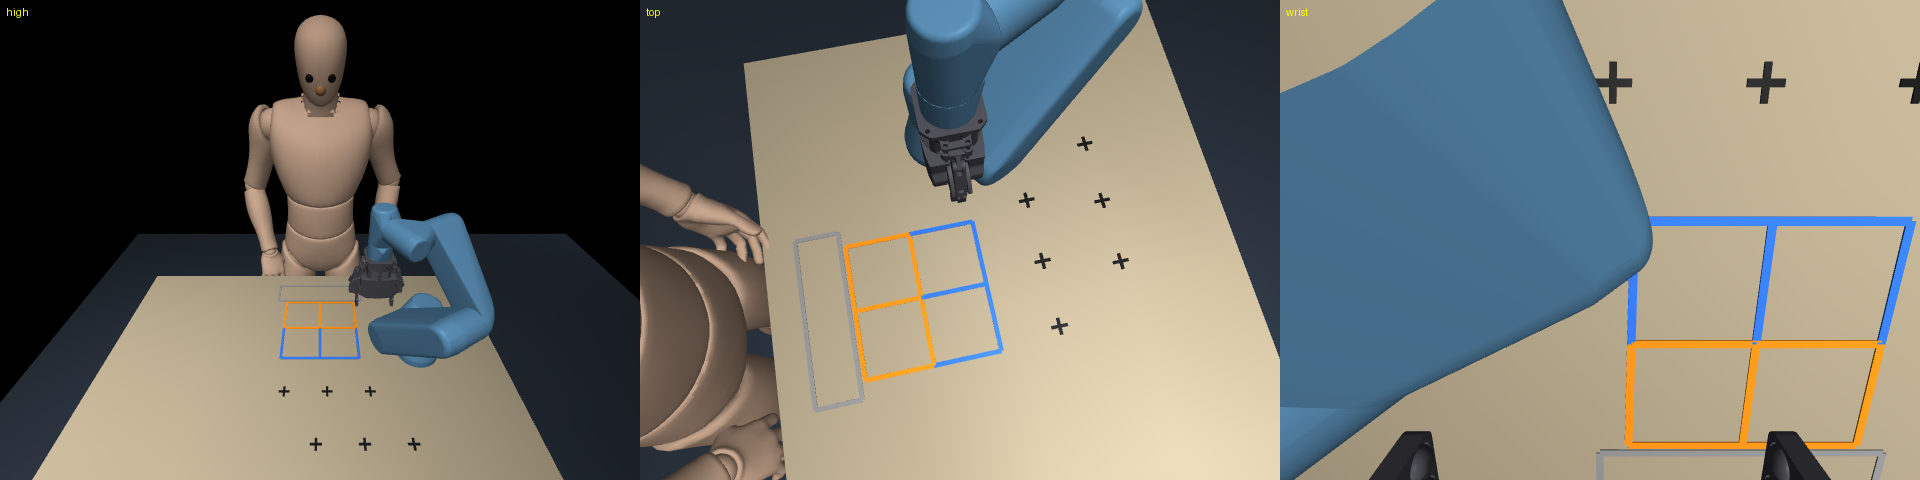
\includegraphics[width=\textwidth]{cameras}
  \caption{Ba góc camera của chính sách: \texttt{high} (trái), \texttt{top} (giữa) và \texttt{wrist} (phải).}
  \label{fig:cameras}
\end{figure}

\section{Bố trí bàn làm việc theo tầm với}
\label{sec:layout}

Người đứng ở mép bàn bên phải robot theo bố trí chéo $90^\circ$, lệch sang bên 0,30~m so với đế robot. Bàn được chia thành các vùng theo khả năng với tới. Tính từ phía người ra xa (Hình~\ref{fig:layout}):
\begin{itemize}
  \item \textbf{Vùng U} (chỉ người với tới): một dải $30\times8$~cm ngay trước người. Nửa phải là chỗ để hai khối mà người tự lấy trong nhiệm vụ T3; nửa trái (\texttt{U\_cup}) là chỗ robot đặt cốc.
  \item \textbf{Hàng H} (vùng chung): hai vùng trao vật H1, H2, nơi lòng bàn tay người nhận vật ở độ cao 15~cm trên mặt bàn.
  \item \textbf{Hàng P} (vùng chung): hai vùng đặt vật P1, P2.
  \item \textbf{Vùng robot}: hai hàng ô vật thẳng, mỗi hàng ba ô cách nhau 12~cm. Hàng gần là S4--S6, hàng xa là S1--S3, hai hàng lệch nhau 3~cm.
\end{itemize}

Bố trí được kiểm tra tự động theo các tiêu chí sau:
\begin{itemize}
  \item mọi vị trí robot cần chạm tới nằm trong bán kính hiệu dụng $R_\text{eff} = 0{,}40$~m, và robot gắp thành công 5/5 lần ở mọi vị trí;
  \item người với tới mọi vùng H, U và chỉ tới mọi ô P, S với độ nghiêng lưng không quá $30^\circ$;
  \item tia chỉ tay tới hai ô S bất kỳ lệch nhau ít nhất $5^\circ$, để mục tiêu của cử chỉ chỉ tay luôn phân biệt được về hình học.
\end{itemize}

\begin{figure}[htbp]
  \centering
  \begin{subfigure}{0.49\textwidth}
    \centering
    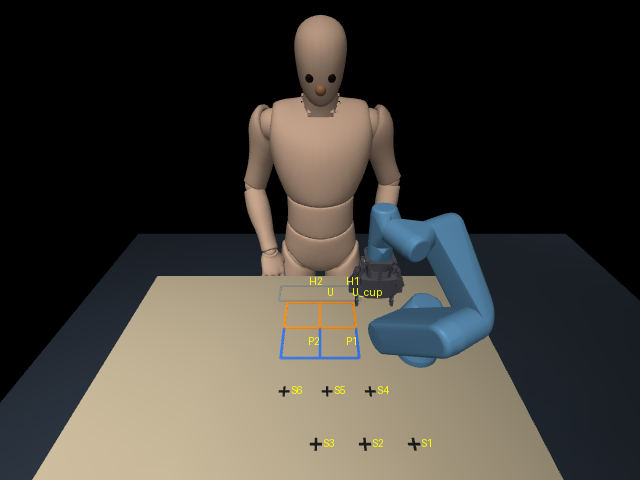
\includegraphics[width=\linewidth]{scene_overview}
    \caption{}
  \end{subfigure}\hfill
  \begin{subfigure}{0.49\textwidth}
    \centering
    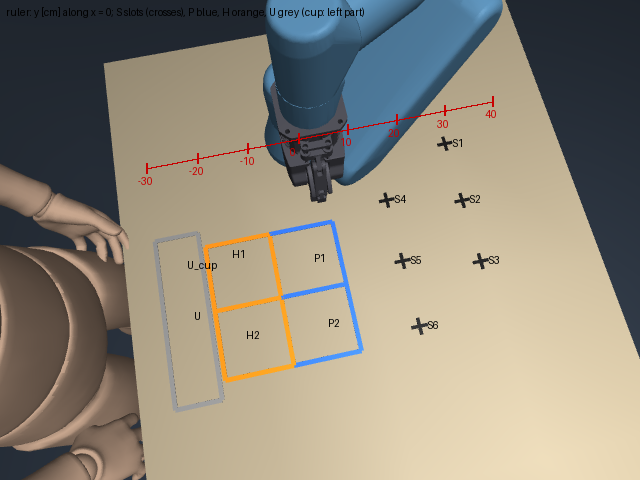
\includegraphics[width=\linewidth]{layout_top}
    \caption{}
  \end{subfigure}
  \caption{Bố trí bàn làm việc: (a) toàn cảnh từ camera \texttt{high}; (b) nhìn từ trên xuống với các ô vật S1--S6 (dấu chữ thập), vùng đặt P (xanh), vùng trao vật H (cam) và vùng người U (xám).}
  \label{fig:layout}
\end{figure}

\paragraph{Bộ vật.} Bộ vật gồm:
\begin{itemize}
  \item ba khối lập phương 4~cm màu đỏ (B1), xanh dương (B2) và vàng (B3);
  \item khối B1$'$ giống hệt B1, dùng để tạo tình huống mơ hồ mà chỉ cử chỉ mới phân biệt được;
  \item hai cốc trắng giống hệt nhau C1, C2 và một cốc xanh lá C3.
\end{itemize}
Mỗi episode đặt 3--4 vật trên bàn (riêng T4 chỉ có 1 khối).

\section{Mô hình người}
\label{sec:human}

Người trong mô phỏng là ma-nơ-canh của HY-Motion~1.0~\cite{wen2025hymotion}, dùng khung xương SMPL-H~\cite{romero2017mano}, được tách thành các đoạn cứng. Hành vi của người được \emph{lập trình sẵn} và tất định theo seed:
\begin{itemize}
  \item \textbf{Quỹ đạo.} Chỉ lòng bàn tay được điều khiển theo quỹ đạo min-jerk~\cite{flash1985minjerk}. Toàn thân được suy ra bằng động học ngược hai khâu cho cánh tay chủ động; thân người cúi ở eo vừa đủ để với tới.
  \item \textbf{Hình bàn tay.} Bàn tay có bốn hình cơ bản (tự nhiên, chỉ, nắm, ngửa đón) cùng các hình trung gian, nên ngón tay chuyển dáng mượt trong khoảng 0,2~s.
  \item \textbf{Chỉ tay.} Khi chỉ tay, cổ tay được ngắm sao cho tia ngón trỏ đi qua đúng mục tiêu, sai lệch dưới 2~cm, và cử chỉ được giữ 1,8--2,5~s (Hình~\ref{fig:human-poses}).
  \item \textbf{Va chạm.} Hình học người chỉ dùng để hiển thị. Va chạm và vi phạm khoảng cách an toàn được đo bằng khoảng cách tới các khối proxy ẩn (lòng bàn tay, cẳng tay, cánh tay trên, thân, đầu).
\end{itemize}

Việc người không phản ứng với robot là một giới hạn có chủ đích. Nhờ đó chuyển động của người \emph{giống hệt nhau} giữa các mô hình được so sánh, giống cách HRIBench cố định lịch xuất hiện của người~\cite{liu2026hribench}. Đây cũng là điều kiện để nguồn ý định \emph{hindsight}, vốn biết trước tương lai, được định nghĩa một cách hợp lệ.

\begin{figure}[htbp]
  \centering
  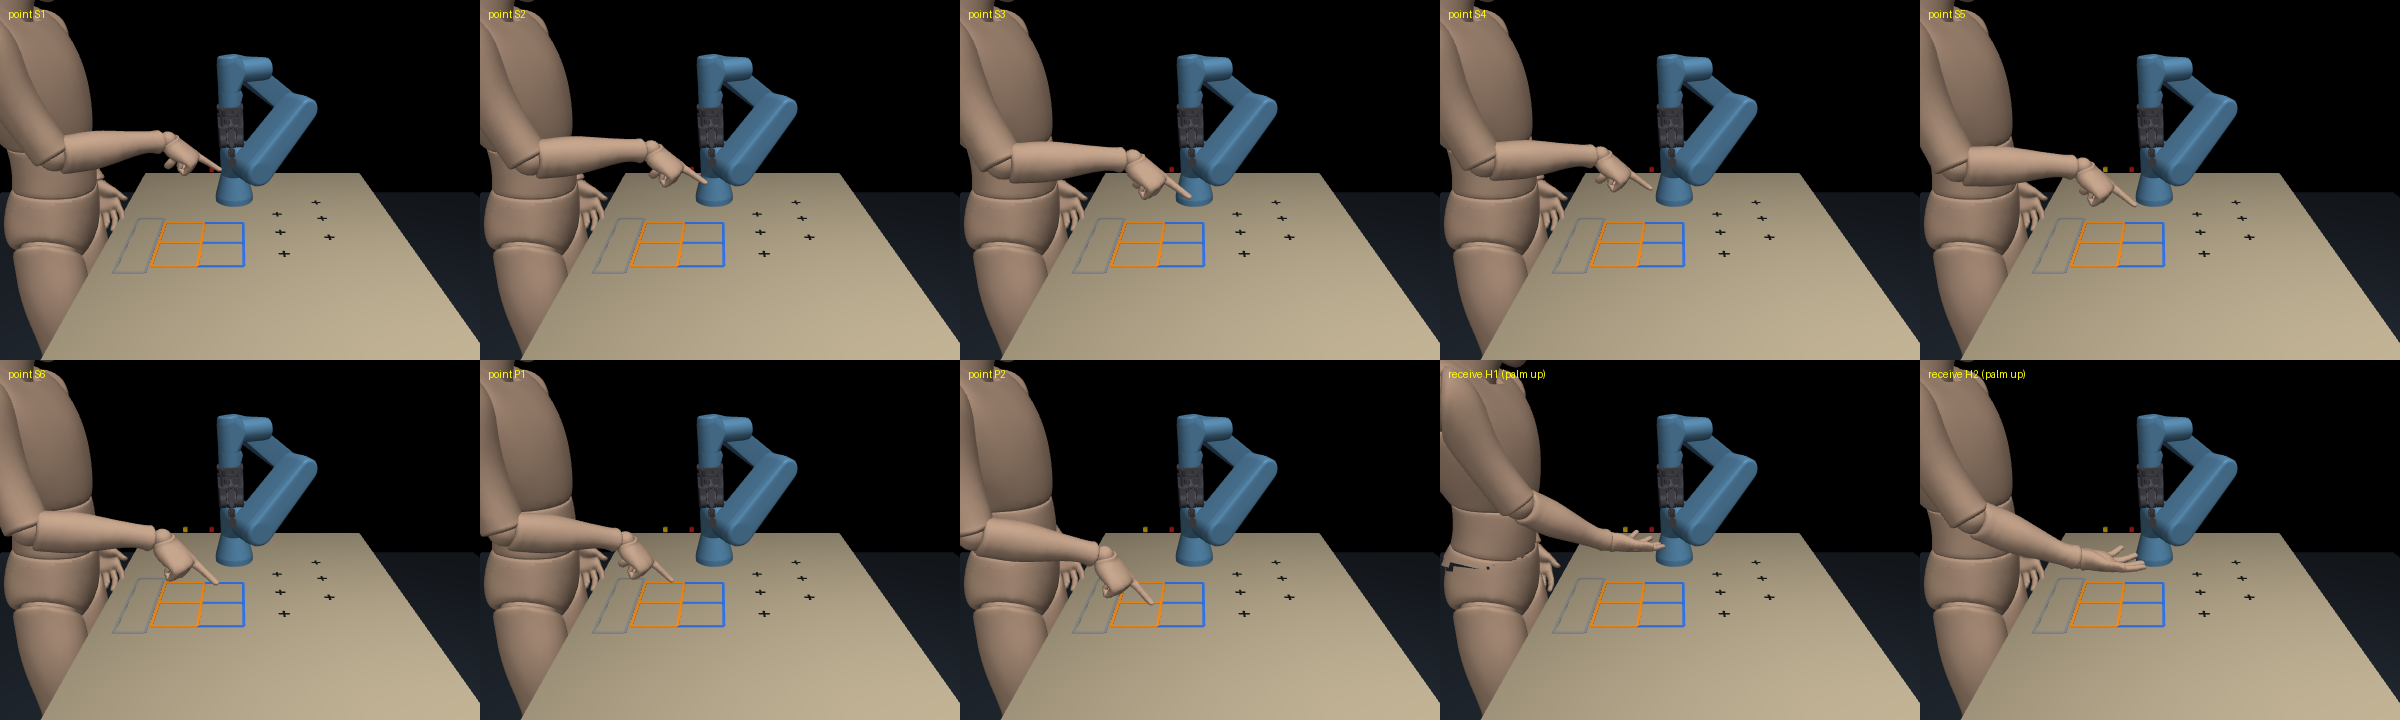
\includegraphics[width=\textwidth]{human_poses}
  \caption{Các cử chỉ của người trong mô phỏng: chỉ tới sáu ô vật S1--S6 và hai vùng đặt P1, P2, và ngửa lòng bàn tay nhận vật ở hai vùng H1, H2.}
  \label{fig:human-poses}
\end{figure}

\section{Bộ bối cảnh nhiệm vụ}
\label{sec:tasks}

Bộ nhiệm vụ gồm năm nhiệm vụ T1--T5 và một biến thể âm T4-neg, thuộc ba vai tương tác như HRIBench~\cite{liu2026hribench}. Bảng~\ref{tab:tasks} tóm tắt các nhiệm vụ.

\begin{table}[htbp]
  \centering
  \caption{Bộ bối cảnh nhiệm vụ.}
  \label{tab:tasks}
  \small
  \begin{tabularx}{\textwidth}{@{}l l X X@{}}
    \toprule
    \textbf{Nhiệm vụ} & \textbf{Vai} & \textbf{Hành vi của người} & \textbf{Robot cần làm / thành công khi} \\
    \midrule
    T1 gắp -- đặt & Instructor & Chỉ vào khối mục tiêu, rồi chỉ vào vùng đặt P & Gắp đúng khối, đặt vào đúng vùng P, về tư thế nghỉ; không chạm vật khác \\
    \addlinespace
    T2 trao vật & Collaborator & Chỉ vào vật, rồi ngửa tay ở một vùng H theo một trong ba thời điểm: sớm, đúng lúc, muộn & Mang đúng vật tới tay đang chờ, giữ yên, chỉ nhả khi người đã cầm \\
    \addlinespace
    T3 hỗ trợ & Collaborator & Không chỉ tay; tự lấy một trong hai khối ở U, mỗi khối gắn với một cốc & Đoán từ việc người với tới khối nào để mang đúng cốc tới \texttt{U\_cup} kịp lúc \\
    \addlinespace
    T4 xâm nhập & Intruder & Đưa tay vào vùng robot ở một trong ba pha (tiến tới vật, mang vật, sắp đặt), giữ 1, 2 hoặc 4~s & Tự gắp -- đặt một khối; dừng khi tay ở trong vùng, tiếp tục đúng chỗ đang dở, không va chạm \\
    \addlinespace
    T4-neg & Intruder & Tay đi gần nhưng ở ngoài vùng robot & Không được dừng không cần thiết \\
    \addlinespace
    T5 đổi ý & theo T1/T2/T3 & Ra hiệu mục tiêu cũ, rút tay, rồi ra hiệu mục tiêu mới; sớm hoặc muộn, luôn trước khi robot gắp & Hoàn thành nhiệm vụ gốc với mục tiêu mới, không chạm vật cũ \\
    \bottomrule
  \end{tabularx}
\end{table}

Mỗi nhiệm vụ kiểm tra một khía cạnh khác nhau của thông tin ý định:
\begin{itemize}
  \item T1 cần thông tin \emph{không gian} (vật nào, đặt ở đâu); trong một phần ba số episode có hai khối giống hệt nhau, nên chỉ cử chỉ mới phân biệt được.
  \item T2 cần thông tin \emph{thời gian}: robot phải tới vùng H đúng lúc tay người sẵn sàng.
  \item T3 là một ``quy trình đã học'': mục tiêu được suy ra từ chuyển động vươn tay chứ không từ cử chỉ chỉ dẫn, nên kiểm tra khả năng đoán sớm.
  \item T4 và T4-neg kiểm tra phản ứng an toàn và khả năng phân biệt xâm nhập thật với chuyển động lân cận vô hại.
  \item T5 kiểm tra khả năng cập nhật mục tiêu khi người đổi ý.
\end{itemize}

\paragraph{Danh sách kịch bản.} Mỗi episode được mô tả bởi:
\begin{itemize}
  \item một \emph{spec} rời rạc: nhiệm vụ, vật mục tiêu, bố trí ô, vùng P/H, có cặp vật giống nhau hay không, thời điểm, pha xâm nhập, đổi ý;
  \item các biến thiên liên tục lấy từ seed: lệch vị trí, thời gian của người.
\end{itemize}
Các spec được sinh thành danh sách cân bằng với seed cố định: mọi tổ hợp biến thể chính xuất hiện gần đều nhau, và hai episode liên tiếp không có cùng ô mục tiêu. Có hai danh sách:
\begin{itemize}
  \item \textbf{Danh sách trình diễn} gồm 280 episode: T1 60, T2 50, T3 60, T4 40, T4-neg 10, T5 60.
  \item \textbf{Danh sách đánh giá} gồm 20 episode mỗi nhiệm vụ (120 episode), với seed khác hẳn danh sách trình diễn. Danh sách này được dùng lại y hệt cho mọi mô hình được so sánh.
\end{itemize}

\section{Expert và dữ liệu trình diễn}
\label{sec:expert}

Dữ liệu trình diễn được sinh bởi một expert lập trình sẵn. Expert có thông tin đặc quyền về ý định thật của người, chỉ dùng để sinh dữ liệu và không bao giờ dùng khi đánh giá chính sách. Expert có ba chế độ thời điểm kích hoạt:
\begin{itemize}
  \item \texttt{cue\_complete} --- \textbf{phản hồi khi ý định đã rõ}: robot chỉ hành động khi người đã ra hiệu xong (ở T3, khi người đã nhấc khối lên).
  \item \texttt{evidence} --- \textbf{phản hồi sớm}:
    \begin{itemize}
      \item robot bắt đầu chuẩn bị (không phụ thuộc mục tiêu) từ lúc người bắt đầu cử chỉ;
      \item robot cam kết hướng tới mục tiêu khi mục tiêu đã đoán được từ cử chỉ, tức ở 40\% chuyển động tiết lộ ý định;
      \item robot chỉ chạm vào vật khi cử chỉ đã được giữ 1,6~s.
    \end{itemize}
  \item \texttt{cue\_onset} --- biết trước ý định ngay từ đầu, chỉ dùng như cận trên tham khảo.
\end{itemize}

Ở T4, robot tự bắt đầu sau 0,5~s trong mọi chế độ. Expert dừng khi tay người ở trong vùng robot (thêm biên 2~cm) hoặc khi lòng bàn tay cách điểm công cụ dưới 12~cm. Ở chế độ phản hồi sớm, expert còn nhường cho vị trí tay được dự đoán trước 0,5~s.

Mỗi bước điều khiển 20~Hz ghi một khung dữ liệu gồm quan sát trước khi hành động và hành động expert đã chọn. Dữ liệu được lưu theo chuẩn LeRobotDataset~v3.0~\cite{cadene2026lerobot}: ảnh nén video, số liệu từng khung ở dạng bảng, và tệp ground truth theo episode (ý định thật, các mốc thời gian, chuyển động của người). Chỉ episode thành công được giữ lại. Từ cùng danh sách 280 kịch bản, hai bộ dữ liệu được thu với hai chế độ expert:
\begin{itemize}
  \item bộ \emph{phản hồi khi rõ} (late): 274 episode, 92\,095 khung;
  \item bộ \emph{phản hồi sớm} (early): 271 episode, 70\,924 khung.
\end{itemize}
Bộ phản hồi sớm ngắn hơn khoảng 23\% về số khung, phản ánh đúng việc robot bắt đầu sớm hơn và ít phải chờ.

% !TEX root = ../main.tex
\chapter[CHÍNH SÁCH HỌC BẮT CHƯỚC NHẬN THỨC Ý ĐỊNH]{CHÍNH SÁCH HỌC BẮT CHƯỚC\\NHẬN THỨC Ý ĐỊNH}
\label{chap:method}

Chương này trình bày phương pháp đề xuất, gồm năm phần:
\begin{itemize}
  \item cách phát biểu bài toán và không gian hành động rút gọn;
  \item cách phân loại thông tin ý định và hợp đồng dữ liệu cố định;
  \item ba nguồn sinh thông tin ý định cùng bộ nhớ mục tiêu dùng chung;
  \item cách đưa thông tin ý định vào ACT;
  \item cách huấn luyện và suy luận.
\end{itemize}

\section{Phát biểu bài toán}
\label{sec:formulation}

Tại mỗi bước điều khiển $t$, chính sách nhận quan sát $o_t$, gồm ba ảnh camera và trạng thái robot $s_t$, cùng nhãn nhiệm vụ $\kappa \in \{\text{T1},\ldots,\text{T4}\}$. Chính sách gốc mô hình hóa phân phối của một đoạn $H$ hành động tương lai:
\begin{equation}
  \pi_\theta\left(a_{t:t+H-1} \mid o_t, \kappa\right).
  \label{eq:policy-base}
\end{equation}

Nhãn nhiệm vụ chỉ cho biết loại nhiệm vụ. Nó không tiết lộ vật mục tiêu, việc người sắp đổi ý, hay việc người có xâm nhập hay không. Vì vậy T5 được gộp vào nhiệm vụ gốc T1/T2/T3, và T4-neg được gộp vào T4. Chính sách nhận thức ý định nhận thêm một vector thông tin ý định $c_t$:
\begin{equation}
  \pi_\theta\left(a_{t:t+H-1} \mid o_t, \kappa, c_t\right).
  \label{eq:policy-intent}
\end{equation}

Câu hỏi trung tâm là liệu \eqref{eq:policy-intent} có tốt hơn \eqref{eq:policy-base} hay không, khi hai mô hình có cùng kiến trúc, cùng dữ liệu và cùng ngân sách huấn luyện.

Một nguyên tắc xuyên suốt: $c_t$ chỉ mô tả \emph{con người}. Không trường nào trong $c_t$ được mã hóa hành động của robot hay thời điểm robot cần bắt đầu. Đó là quyết định của chính sách. Nếu vi phạm nguyên tắc này, chính sách có thể ``chép đáp án'' từ $c_t$, và mọi so sánh sẽ mất ý nghĩa.

\section{Không gian hành động rút gọn}
\label{sec:action-space}

Để đo tác động của ý định một cách rõ ràng nhất, chính sách xuất ra hành động rời rạc trong tập 9 hành động ở Bảng~\ref{tab:actions}, thay vì quỹ đạo khớp liên tục như ACT gốc. Mỗi hành động được ánh xạ tất định thành một điểm đặt Cartesian của điểm công cụ (bước 1~cm trong hệ gốc robot), rồi thành mục tiêu khớp qua động học ngược với hướng kẹp cố định từ trên xuống. Điểm đặt bị giới hạn trong một hộp an toàn, và các điểm đặt mà động học ngược không đạt được sẽ bị từ chối. Tần số ra quyết định là 20~Hz.

\begin{table}[htbp]
  \centering
  \caption{Không gian hành động rút gọn gồm 9 hành động.}
  \label{tab:actions}
  \small
  \begin{tabular}{@{}cll@{}}
    \toprule
    \textbf{Mã} & \textbf{Hành động} & \textbf{Lệnh điều khiển} \\
    \midrule
    0 & \texttt{HOLD} & giữ nguyên điểm đặt \\
    1 / 2 & \texttt{MOVE\_FORWARD} / \texttt{MOVE\_BACKWARD} & $\pm 1$~cm theo $X$ (về phía người / về phía robot) \\
    3 / 4 & \texttt{MOVE\_LEFT} / \texttt{MOVE\_RIGHT} & $\pm 1$~cm theo $Y$ \\
    5 / 6 & \texttt{MOVE\_UP} / \texttt{MOVE\_DOWN} & $\pm 1$~cm theo $Z$ \\
    7 / 8 & \texttt{OPEN\_GRIPPER} / \texttt{CLOSE\_GRIPPER} & khe kẹp 0,085~m / 0~m \\
    \bottomrule
  \end{tabular}
\end{table}

Việc rút gọn mang lại ba lợi ích:
\begin{itemize}
  \item Hành động của chính sách và của expert so sánh được trực tiếp bằng argmax, nhờ đó định nghĩa được các chỉ số ``hành động có đổi không'' và ``đổi có đúng không'' ở Mục~\ref{sec:offline-checks}.
  \item Đầu phân loại cho ra log-xác suất của từng hành động, thuận tiện cho phân tích.
  \item Độ khó điều khiển mức thấp được loại bỏ, để sự khác biệt giữa các mô hình chủ yếu đến từ việc \emph{chọn đúng việc cần làm và đúng lúc}.
\end{itemize}

\section{Phân loại thông tin ý định}
\label{sec:intent-taxonomy}

Để phối hợp với người, robot cần trả lời năm câu hỏi: \emph{làm gì} (what), \emph{ai làm} (who), \emph{vật nào} (which), \emph{ở đâu} (where) và \emph{khi nào} (when). Mỗi câu hỏi được đáp ứng bởi một loại thông tin (Bảng~\ref{tab:taxonomy}):
\begin{itemize}
  \item \textbf{ngữ nghĩa}: nhiệm vụ và vai trò;
  \item \textbf{không gian}: mục tiêu và vùng người chiếm;
  \item \textbf{thời gian}: thời điểm người hoàn thành cử chỉ.
\end{itemize}

Thông tin thời gian là nơi \emph{dự đoán} có giá trị nhất. Khi biết trước người sẽ hoàn thành cử chỉ sau bao lâu, robot có thời gian để chuẩn bị thay vì chờ tới khi mọi thứ đã rõ.

\begin{table}[htbp]
  \centering
  \caption{Câu hỏi HRI, loại thông tin và trường tương ứng trong hợp đồng dữ liệu.}
  \label{tab:taxonomy}
  \begin{tabularx}{\textwidth}{@{}l l X@{}}
    \toprule
    \textbf{Câu hỏi} & \textbf{Loại thông tin} & \textbf{Trường} \\
    \midrule
    Làm gì (what) & ngữ nghĩa & \texttt{task\_id} (cài sẵn) \\
    Ai làm (who) & ngữ nghĩa, suy ra từ loại cử chỉ & \texttt{p\_who}, \texttt{c\_who} \\
    Vật nào, ở đâu (which, where) & không gian & \texttt{p\_target}, \texttt{c\_target}, \texttt{occupancy} \\
    Khi nào (when) & thời gian & \texttt{tte}, \texttt{tte\_std}, \texttt{phase} \\
    Như thế nào (how) & không gian và thời gian & \texttt{xi} \\
    \bottomrule
  \end{tabularx}
\end{table}

\section{Hợp đồng dữ liệu ý định}
\label{sec:contract}

Một rủi ro lớn khi đưa thông tin ý định vào chính sách là chính sách ``quen'' với một dạng dữ liệu lý tưởng, rồi bị ``sốc'' khi gặp dữ liệu thật từ một bộ dự đoán. Để tránh điều này, mọi nguồn thông tin ý định phải xuất ra \emph{đúng một hợp đồng dữ liệu cố định}: cùng tên trường, cùng kích thước và cùng miền giá trị (Bảng~\ref{tab:contract}). Chính sách không được biết đang chạy với nguồn nào.

Hợp đồng dùng ba bộ từ vựng:
\begin{itemize}
  \item \textbf{Mục tiêu}: $K = 17$ \emph{vị trí} theo thứ tự cố định: \texttt{none}, S1--S6, U1, U2, U, P1, P2, H1, H2, \texttt{U\_cup}, \texttt{robot\_zone}, \texttt{zone\_edge}. Mục tiêu là vị trí chứ không phải danh tính vật, vì các vật giống hệt nhau đứng ở ô ngẫu nhiên.
  \item \textbf{Vai trò}: \texttt{[none, robot, human, joint]}.
  \item \textbf{Pha cử chỉ}: \texttt{[rest, prepare, stroke, hold, retract]}.
\end{itemize}

Quỹ đạo tay tương lai \texttt{xi} gồm $M = 8$ mốc cách đều trong 1,2~s tới, cho $J = 6$ keypoint: cổ tay, gốc ngón trỏ và đầu ngón trỏ của mỗi tay.

\begin{table}[htbp]
  \centering
  \caption{Hợp đồng dữ liệu ý định. Tiền tố \texttt{p\_} là thông tin tức thời, cập nhật mỗi khung; tiền tố \texttt{c\_} là thông tin đã chốt, do bộ nhớ mục tiêu giữ tới khi hoàn thành.}
  \label{tab:contract}
  \small
  \begin{tabularx}{\textwidth}{@{}l l X@{}}
    \toprule
    \textbf{Trường} & \textbf{Kích thước} & \textbf{Ý nghĩa và ràng buộc} \\
    \midrule
    \texttt{p\_who} & 4 & phân phối vai trò của cử chỉ hiện tại, tổng bằng 1 \\
    \texttt{p\_target} & $K$ & phân phối mục tiêu tức thời; không có ý định thì dồn vào \texttt{none} \\
    \texttt{c\_who}, \texttt{c\_target} & 4, $K$ & vai trò và mục tiêu đã chốt; \texttt{none} khi chưa chốt \\
    \texttt{occupancy} & 7 & hộp bao vùng tay người sắp chiếm $[c_x, c_y, c_z, s_x, s_y, s_z, \text{conf}]$ (mét) \\
    \texttt{tte} & 1 & thời gian tới khi cử chỉ đạt tư thế đích, $[0, 3]$~s \\
    \texttt{tte\_std} & 1 & độ bất định của \texttt{tte} \\
    \texttt{phase} & 5 & phân phối pha cử chỉ \\
    \texttt{xi} & $M \times J \times 3$ & vị trí keypoint tay tương lai, \emph{tương đối} vị trí hiện tại, hệ gốc robot \\
    \texttt{confidence} & 2 & $\left[1 - H(\texttt{p\_target})/\log K,\ \max \texttt{p\_who}\right]$ \\
    \bottomrule
  \end{tabularx}
\end{table}

Hợp đồng có ba ràng buộc bắt buộc:
\begin{itemize}
  \item Không phân phối nào được là vector toàn 0; trạng thái ``không có gì'' luôn dồn vào lớp \texttt{none}.
  \item Mọi phân phối có tổng bằng 1 với sai số $10^{-4}$.
  \item Không có giá trị NaN.
\end{itemize}
Một hàm kiểm tra được gọi cả khi ghi dữ liệu lẫn trong bộ kiểm thử.

\paragraph{Mốc thời gian của một cử chỉ.} Mỗi cử chỉ mang ý định của người tạo một đoạn với các mốc sau, tương tự cách Ego4D và Ortenzi và cộng sự phân pha hành động~\cite{grauman2022ego4d,ortenzi2021handovers}:
\begin{itemize}
  \item $t_\text{onset}$: người bắt đầu chuyển động tay của cử chỉ;
  \item $t_\text{clear}$: chuyển động kết thúc, cử chỉ đã thành hình và ý định trở nên rõ ràng;
  \item $t_\text{event}$: cử chỉ kết thúc, tính cả thời gian giữ;
  \item $t_\text{end}$: kết thúc các giai đoạn ``chờ robot'' sau đó, ví dụ tay đưa ra chờ nhận vật.
\end{itemize}
Điểm cam kết 40\% mà expert phản hồi sớm sử dụng nằm giữa $t_\text{onset}$ và $t_\text{clear}$.

\section{Các nguồn thông tin ý định}
\label{sec:sources}

Ba nguồn cùng cài đặt một giao diện: tại mỗi bước, nguồn nhận keypoint của người và trạng thái robot, rồi trả về đúng hợp đồng ở Bảng~\ref{tab:contract}. Ba nguồn khác nhau ở mức độ ``lý tưởng'' của thông tin. Nhờ đó tách được giá trị của bản thân thông tin khỏi chất lượng của bộ dự đoán.

\subsection{Nguồn hindsight}

Nguồn hindsight đọc trực tiếp các đoạn ground truth của mô phỏng:
\begin{itemize}
  \item \texttt{p\_target} và \texttt{p\_who} là one-hot đúng trong $[t_\text{onset}, t_\text{end}]$ và là \texttt{none} ngoài khoảng đó;
  \item \texttt{tte} và \texttt{phase} tính từ các mốc thật;
  \item \texttt{xi} là vị trí tay tương lai thật.
\end{itemize}
Nguồn này \emph{biết tương lai}, nên chỉ đóng vai trò cận trên của lợi ích có thể đạt được, không dùng cho mô hình triển khai thật. Nó chỉ hợp lệ khi chuyển động của người không phụ thuộc robot, đúng như thiết lập ở Mục~\ref{sec:human}.

\subsection{Nguồn perfect}

Nguồn perfect hoàn toàn \emph{nhân quả}: tại thời điểm $t$ chỉ dùng dữ liệu tới $t$, trên keypoint sạch. Nó không dùng các mốc ground truth $t_\text{onset}$, $t_\text{clear}$. Nguồn này kết hợp hai bằng chứng về mục tiêu.

\paragraph{Tia chỉ tay.} Tia chỉ tay đi từ gốc ngón trỏ qua đầu ngón trỏ. Với góc lệch $\theta_k$ từ tia tới tâm ô $k$, bằng chứng chỉ tay là
\begin{equation}
  p_\text{point}(k) \propto \exp\left(-\frac{\theta_k^2}{2\sigma^2}\right),
  \label{eq:point}
\end{equation}
và chỉ bật khi cử chỉ là chỉ tay. Độ rộng $\sigma = 4{,}61^\circ$ không phải giá trị chọn tay mà là phân vị 95\% của sai số góc đo được trên dữ liệu (Mục~\ref{sec:source-quality}).

\paragraph{Điểm cuối quỹ đạo.} Vị trí tay tương lai được ngoại suy bằng mô hình vận tốc không đổi~\cite{scholler2020cvm}, sau khi làm mượt bằng bộ lọc Savitzky--Golay~\cite{savitzky1964}. Điểm cuối tại 1,2~s được chuyển thành phân phối $p_\text{reach}$ qua softmax của khoảng cách tới từng ô, với nhiệt độ 5~cm.

\paragraph{Gộp Bayes theo thời gian.} Hai bằng chứng được gộp đệ quy:
\begin{equation}
  p_t(k) \propto \left[\textstyle\sum_j T_{jk}\, p_{t-1}(j)\right] \cdot p_\text{point}(k)^{w_1} \cdot p_\text{reach}(k)^{w_2},
  \label{eq:bayes}
\end{equation}
với $T$ là ma trận chuyển có xác suất ở lại $1-\varepsilon$ ($\varepsilon = 0{,}02$), cho phép người đổi ý.

\paragraph{Các trường còn lại.} Các trường còn lại được tính như sau:
\begin{itemize}
  \item \textbf{Loại cử chỉ.} Thời điểm bắt đầu cử chỉ được phát hiện bằng ngưỡng tốc độ tay (0,08~m/s). Xác suất của lớp cử chỉ đúng tăng tuyến tính tới 0,95 sau $1{,}15$~s, là trung vị của $t_\text{clear} - t_\text{onset}$ đo trên tập huấn luyện. Vai trò được suy ra từ cử chỉ: chỉ tay $\to$ robot làm, vươn tay $\to$ người làm, ngửa tay ở vùng H $\to$ cùng làm.
  \item \textbf{\texttt{tte}.} Bằng khoảng cách tới tư thế đích của cử chỉ chia cho tốc độ tay.
  \item \textbf{\texttt{phase}.} Theo luật động học: tốc độ, khoảng cách tới đích, thời gian giữ yên.
  \item \textbf{\texttt{occupancy}.} Là hộp bao quanh \texttt{xi} cộng biên 5~cm.
\end{itemize}

\subsection{Nguồn predicted}

Nguồn predicted chạy cùng đường ống với nguồn perfect, nhưng khác ở hai điểm:
\begin{itemize}
  \item \textbf{Keypoint có nhiễu.} Keypoint đi qua một mô hình nhiễu (rung, mất tay, trễ, lệch góc). Tham số của mô hình nhiễu được thiết kế để đo từ dữ liệu người thật ghi bằng camera RGB-D và MediaPipe~\cite{zhang2020mediapipe}.
  \item \textbf{Cử chỉ do mô hình học được.} Loại cử chỉ do một bộ phân loại nhỏ huấn luyện trên chuỗi keypoint dự đoán. Bộ phân loại được huấn luyện theo \emph{cross-fitting} năm phần: mỗi phần của tập huấn luyện được gán nhãn bởi bộ phân loại học trên bốn phần còn lại. Nhờ đó chính sách thấy đúng loại lỗi mà bộ dự đoán mắc phải ngoài tập huấn luyện của nó. Xác suất đầu ra được hiệu chỉnh bằng temperature scaling~\cite{guo2017calibration}.
\end{itemize}
Bộ dự báo chuyển động mặc định là mô hình vận tốc không đổi, với giao diện để thay bằng các mô hình học được như siMLPe hay InteRACT~\cite{guo2023simlpe,kedia2024interact}.

\subsection{Bộ nhớ mục tiêu (IntentTracker)}
\label{sec:tracker}

ACT không có bộ nhớ: mỗi quyết định chỉ dựa trên quan sát hiện tại. Trong T1, người chỉ vào khối rồi chỉ vào vùng đặt, sau đó hạ tay về. Khi robot bắt đầu gắp, thông tin tức thời \texttt{p\_target} đã trở về \texttt{none}. Bộ nhớ mục tiêu giải quyết vấn đề này bằng cách giữ các mục tiêu đã chốt trong một hàng đợi, theo các luật sau:
\begin{itemize}
  \item \textbf{Chốt.} Khi $\max \texttt{p\_target} \geq 0{,}8$ và cử chỉ ổn định ít nhất 5 khung, một cặp (vai trò, mục tiêu) được đưa vào hàng đợi theo văn phạm:
    \begin{itemize}
      \item chỉ vào ô vật $\to$ robot gắp;
      \item chỉ vào ô đặt $\to$ robot đặt, chỉ khi đã có lệnh gắp chờ hoặc đang cầm vật;
      \item ngửa tay ở vùng H $\to$ trao vật.
    \end{itemize}
  \item \textbf{Thay thế.} Chỉ vào một ô vật khác khi vật cũ chưa được gắp sẽ \emph{thay thế} mục tiêu cũ. Đây là cách xử lý người đổi ý (T5).
  \item \textbf{Hoàn thành.} Mục tiêu đầu hàng được lấy ra khi trạng thái robot cho thấy bước đó đã xong:
    \begin{itemize}
      \item gắp xong: kẹp đóng, đang giữ vật và đã nâng quá 3~cm;
      \item đặt xong: kẹp mở trong bán kính 8~cm quanh ô đích;
      \item trao xong: kẹp mở khi tay người ở gần vùng H.
    \end{itemize}
\end{itemize}

Cờ ``đang giữ vật'' được suy ra từ độ mở kẹp đo được chứ không đọc từ mô phỏng, để bộ nhớ dùng được trên robot thật.

Bộ nhớ dùng chung cho cả ba nguồn. Với nguồn hindsight, nó nhận sự kiện ground truth thay cho các phân phối. T3 và T4 không có luật chốt, vì mục tiêu ở đó được suy ra từ chuyển động chứ không từ chỉ dẫn, nên các trường \texttt{c\_} luôn là \texttt{none} ở hai nhiệm vụ này.

\section{Đưa thông tin ý định vào ACT}
\label{sec:intent-act}

\subsection{Kiến trúc}

Chính sách được xây dựng trên lớp ACT của LeRobot~\cite{cadene2026lerobot}, không sửa thư viện gốc. Mỗi ảnh camera đi qua ResNet18~\cite{he2016resnet} khởi tạo từ ImageNet, cho một lưới token ảnh. Trạng thái robot cho một token. Nhãn nhiệm vụ và thông tin ý định được chiếu thành 14 token và chèn vào chuỗi đầu vào của bộ mã hóa transformer, ngay sau các token một chiều và trước các token ảnh (Hình~\ref{fig:intent-act}). Các token ý định gồm:
\begin{itemize}
  \item \textbf{TASK}: \texttt{Embedding} của nhãn nhiệm vụ. Token này có ở \emph{mọi} mô hình, kể cả mô hình gốc.
  \item \textbf{WHO}: \texttt{p\_who} $\oplus$ \texttt{c\_who} qua một lớp tuyến tính.
  \item \textbf{TARGET} và \textbf{C\_TARGET}: phân phối mục tiêu nhân với một bảng embedding $E_\text{target} \in \mathbb{R}^{K\times d}$ \emph{dùng chung}, để ``ô S3'' có cùng biểu diễn dù là ý định tức thời hay đã chốt. C\_TARGET cộng thêm một embedding vai trò ``đã chốt''.
  \item \textbf{OCC}: \texttt{occupancy} qua một lớp tuyến tính.
  \item \textbf{TIME}: đặc trưng Fourier~\cite{tancik2020fourier} của \texttt{tte}, ghép với độ bất định của \texttt{tte}, phân phối pha và hai giá trị độ tin cậy, qua một MLP.
  \item \textbf{XI$_1$..XI$_8$}: mỗi mốc quỹ đạo tương lai (đã chuẩn hóa z-score theo thống kê tập huấn luyện) qua một lớp tuyến tính, cộng embedding thời gian của mốc.
\end{itemize}
Mỗi token cộng thêm một embedding loại theo nhóm thông tin, và bảng embedding vị trí một chiều của ACT được mở rộng tương ứng. Khi tắt cả token nhiệm vụ lẫn token ý định, mô hình trùng khớp với ACT gốc; điều này được kiểm tra bằng bộ kiểm thử tự động.

\begin{figure}[htbp]
  \centering
  \resizebox{\linewidth}{!}{%
  \begin{tikzpicture}[
      font=\small,
      box/.style={draw, rounded corners=2pt, align=center, minimum height=0.9cm, inner sep=4pt},
      tok/.style={draw, fill=#1, minimum width=0.55cm, minimum height=0.55cm, inner sep=0pt, font=\scriptsize},
      tok/.default=white,
      arr/.style={-{Latex[length=2mm]}, thick}]
    % inputs
    \node[box, fill=gray!10] (img) at (0,0) {3 ảnh camera\\$256\times192$};
    \node[box, fill=gray!10] (state) at (0,-1.6) {trạng thái\\robot $s_t$};
    \node[box, fill=orange!15] (intent) at (0,-3.4) {thông tin ý định $c_t$\\(hợp đồng dữ liệu)};
    \node[box, fill=orange!5] (task) at (0,-5.0) {nhãn nhiệm vụ $\kappa$};
    % encoders
    \node[box] (resnet) at (3.3,0) {ResNet18};
    \node[box] (lin) at (3.3,-1.6) {Linear};
    \node[box, fill=orange!15] (ienc) at (3.3,-3.4) {bộ mã hóa\\ý định};
    \node[box, fill=orange!5] (temb) at (3.3,-5.0) {Embedding};
    % tokens column
    \node[tok=gray!10] (ti) at (6.0,0) {};
    \node[tok=gray!10, right=0pt of ti] (ti2) {};
    \node[tok=gray!10, right=0pt of ti2] (ti3) {$\cdots$};
    \node[tok=gray!10] (ts) at (6.0,-1.6) {};
    \node[tok=orange!15] (w) at (6.0,-3.4) {W};
    \node[tok=orange!15, right=0pt of w] (t1) {T};
    \node[tok=orange!15, right=0pt of t1] (t2) {C};
    \node[tok=orange!15, right=0pt of t2] (t3) {O};
    \node[tok=orange!15, right=0pt of t3] (t4) {$\tau$};
    \node[tok=orange!15, right=0pt of t4] (t5) {$\xi{\times}8$};
    \node[tok=orange!5] (tt) at (6.0,-5.0) {K};
    % transformer
    \node[box, minimum width=2.4cm, minimum height=5.8cm, fill=blue!5] (enc) at (10.6,-2.5) {Transformer\\mã hóa\\(4 lớp)\\[6pt]$\downarrow$\\[6pt]Transformer\\giải mã\\(1 lớp)};
    \node[box, fill=blue!10] (head) at (13.4,-2.5) {đầu phân loại\\$H\times 9$\\hành động};
    % arrows
    \draw[arr] (img) -- (resnet);  \draw[arr] (resnet) -- (ti);
    \draw[arr] (state) -- (lin);   \draw[arr] (lin) -- (ts);
    \draw[arr] (intent) -- (ienc); \draw[arr] (ienc) -- (w);
    \draw[arr] (task) -- (temb);   \draw[arr] (temb) -- (tt);
    \draw[arr] (ti3.east) -- (ti3.east -| enc.west);
    \draw[arr] (ts.east) -- (ts.east -| enc.west);
    \draw[arr] (t5.east) -- (t5.east -| enc.west);
    \draw[arr] (tt.east) -- (tt.east -| enc.west);
    \draw[arr] (enc) -- (head);
    \node[font=\scriptsize, align=center] at (7.15,-4.15) {dropout theo nhóm\\(token rỗng học được)};
  \end{tikzpicture}}
  \caption{Kiến trúc chính sách nhận thức ý định. Thông tin ý định được chiếu thành các token WHO (W), TARGET (T), C\_TARGET (C), OCC (O), TIME ($\tau$) và 8 token XI ($\xi$), rồi đưa chung vào bộ mã hóa transformer của ACT cùng token nhiệm vụ (K), token trạng thái và token ảnh.}
  \label{fig:intent-act}
\end{figure}

\subsection{Đầu ra và hàm mất mát}

Đầu ra của bộ giải mã cho mỗi vị trí trong đoạn $H$ bước được chiếu thành 9 logit. Hàm mất mát là cross-entropy trung bình trên các vị trí hợp lệ của đoạn (bỏ qua phần đệm ở cuối episode). Vì dùng đầu phân loại, nhánh CVAE của ACT không cần thiết và được tắt.

\subsection{Dropout theo nhóm thông tin}
\label{sec:group-dropout}

Các token ý định được chia thành năm nhóm:
\begin{itemize}
  \item \emph{ngữ nghĩa}: WHO;
  \item \emph{không gian}: TARGET, OCC;
  \item \emph{bộ nhớ}: C\_TARGET;
  \item \emph{thời gian}: TIME;
  \item \emph{chuyển động}: XI.
\end{itemize}
Khi huấn luyện, mỗi nhóm bị thay bằng \emph{token rỗng học được}, riêng cho từng token, với xác suất 0,15. Toàn bộ thông tin ý định bị thay với xác suất 0,1. Cách làm này tương tự dropout mục tiêu của BESO~\cite{reuss2023beso} và classifier-free guidance~\cite{ho2022cfg}, và có hai tác dụng:
\begin{itemize}
  \item chống việc chính sách phụ thuộc hoàn toàn vào một nhóm;
  \item cho phép đánh giá cùng một mô hình khi chỉ giữ lại một tập con các nhóm, phục vụ câu hỏi ``loại thông tin nào hữu ích'' (Mục~\ref{sec:research-questions}).
\end{itemize}
Token rỗng học được được ưu tiên hơn vector 0, vì vector 0 cộng embedding vị trí vẫn là một token ``có nghĩa''.

\subsection{Suy luận}

Chính sách tính lại quyết định ở mọi bước (thực thi 1 hành động mỗi lần dự đoán, không dùng temporal ensembling). Thực thi nhiều bước của một đoạn làm tăng quán tính, khiến robot chậm phản ứng với người, và theo Xu và cộng sự~\cite{xu2026learning} còn làm tăng nguy cơ khởi động sớm sai.

Trong vòng kín, thông tin ý định được tính trực tuyến từ nguồn đã chọn. Một phương án dự phòng là FiLM~\cite{perez2018film}: hệ số $\gamma, \beta$ sinh từ trung bình các token ý định, áp lên bản đồ đặc trưng ảnh, khởi tạo để biến đổi ban đầu là đồng nhất. Phương án này đã được cài đặt nhưng chỉ bật nếu chính sách bỏ qua thông tin ý định.

% !TEX root = ../main.tex
\chapter[THIẾT KẾ THÍ NGHIỆM VÀ QUY TRÌNH ĐÁNH GIÁ]{THIẾT KẾ THÍ NGHIỆM\\VÀ QUY TRÌNH ĐÁNH GIÁ}
\label{chap:experiments}

Chương này trình bày ba nội dung:
\begin{itemize}
  \item thiết kế thí nghiệm $2\times2$ dùng để trả lời các câu hỏi nghiên cứu;
  \item quy trình đánh giá hai mức: kiểm tra ngoại tuyến xem chính sách có \emph{dùng} thông tin ý định hay không, và đánh giá vòng kín bằng các chỉ số tương tác;
  \item thiết lập huấn luyện cụ thể.
\end{itemize}

\section{Thiết kế thí nghiệm \texorpdfstring{$2\times2$}{2×2}}
\label{sec:design-2x2}

Một khó khăn khi đánh giá lợi ích của thông tin ý định là hai yếu tố rất dễ bị lẫn vào nhau:
\begin{itemize}
  \item bản thân \emph{thông tin} ý định;
  \item \emph{thời điểm} robot phản hồi trong dữ liệu trình diễn.
\end{itemize}
Nếu dữ liệu trình diễn chỉ phản hồi khi ý định đã hoàn toàn rõ, thì ảnh camera tại thời điểm đó đã chứa đủ thông tin để hành động, và thông tin ý định hầu như không có gì để đóng góp. Ngược lại, nếu dữ liệu phản hồi sớm, thì chính dữ liệu đã đòi hỏi chính sách phải ``đoán trước''. Khi đó cần biết lợi ích đến từ thông tin ý định hay chỉ từ dữ liệu sớm hơn.

Để tách hai yếu tố, khóa luận huấn luyện bốn mô hình theo thiết kế $2\times2$ (Bảng~\ref{tab:2x2}):
\begin{itemize}
  \item A: không có thông tin ý định; thời điểm phản hồi là khi ý định của người hoàn toàn rõ ràng.
  \item B: không có thông tin ý định; thời điểm phản hồi là trước khi ý định của người hoàn toàn rõ ràng.
  \item C: có thông tin ý định; thời điểm phản hồi là khi ý định của người hoàn toàn rõ ràng.
  \item D: có thông tin ý định; thời điểm phản hồi là trước khi ý định của người hoàn toàn rõ ràng.
\end{itemize}

Hai bộ dữ liệu được thu từ \emph{cùng} danh sách 280 kịch bản, cùng seed, với hai chế độ expert ở Mục~\ref{sec:expert}. A và C dùng chung bộ phản hồi khi rõ; B và D dùng chung bộ phản hồi sớm. Như vậy:
\begin{itemize}
  \item hai mô hình cùng hàng của Bảng~\ref{tab:2x2} chỉ khác nhau ở thời điểm phản hồi của expert;
  \item hai mô hình cùng cột chỉ khác nhau ở việc có nhận thông tin ý định hay không.
\end{itemize}
Mọi mô hình đều có token nhiệm vụ, cùng kiến trúc, cùng siêu tham số và cùng số bước huấn luyện.

\begin{table}[htbp]
  \centering
  \caption{Bốn mô hình của thiết kế thí nghiệm $2\times2$.}
  \label{tab:2x2}
  \begin{tabular}{@{}lcc@{}}
    \toprule
    & \makecell{Phản hồi khi ý định\\hoàn toàn rõ ràng} & \makecell{Phản hồi trước khi ý định\\hoàn toàn rõ ràng} \\
    \midrule
    Không có thông tin ý định & A & B \\
    Có thông tin ý định       & C & D \\
    \bottomrule
  \end{tabular}
\end{table}

\section{Câu hỏi nghiên cứu}
\label{sec:research-questions}

Bốn câu hỏi của Chương~\ref{chap:introduction} tương ứng với bốn phép so sánh:
\begin{itemize}
  \item \textbf{Q1} (A với B): chính sách gốc có khả năng phản ứng sớm với ý định của người không? Nếu B học được hành vi sớm mà không cần thông tin ý định, thì ảnh camera đã chứa đủ tín hiệu để đoán trước.
  \item \textbf{Q2} (A với C): chính sách nhận thức ý định có cải thiện độ chính xác không, trong trường hợp robot chỉ phản hồi khi đã rõ?
  \item \textbf{Q3} (B với D): chính sách nhận thức ý định có khả năng phản ứng sớm tốt hơn chính sách gốc không?
  \item \textbf{Q4} (A với D): câu hỏi chính --- thông tin ý định, cùng với dữ liệu phản hồi sớm, có cải thiện chính sách hành động gốc không?
\end{itemize}

Ngoài thiết kế $2\times2$, khóa luận đặt thêm hai câu hỏi về \emph{cách biểu diễn} thông tin ý định:
\begin{itemize}
  \item \textbf{Loại thông tin nào hữu ích?} Trên cùng mô hình D, chỉ giữ lại một tập con các nhóm thông tin (ngữ nghĩa, không gian, bộ nhớ, thời gian, chuyển động) và thay các nhóm còn lại bằng token rỗng (Mục~\ref{sec:group-dropout}).
  \item \textbf{Lợi ích còn lại bao nhiêu khi thông tin được dự đoán?} Lần lượt thay nguồn hindsight bằng nguồn perfect rồi predicted (Mục~\ref{sec:sources}), và báo cáo khoảng cách giữa các mức.
\end{itemize}

\section{Kiểm tra ngoại tuyến: chính sách có dùng thông tin ý định không?}
\label{sec:offline-checks}

Một chính sách có thể đạt độ chính xác cao mà không hề đọc thông tin ý định, nếu ảnh camera đã đủ để đoán hành động. Vì vậy, trước khi so sánh tỉ lệ thành công, khóa luận kiểm tra trực tiếp xem đầu ra của chính sách có \emph{phụ thuộc} vào thông tin ý định hay không, bằng các can thiệp phản thực tế (counterfactual) trên dữ liệu kiểm định.

Mỗi khung của các episode kiểm định được đánh giá ở các chế độ sau (biến tiềm ẩn bằng 0):
\begin{itemize}
  \item \textbf{gốc}: thông tin ý định đúng;
  \item \textbf{hoán đổi theo nhóm}, luôn bằng giá trị \emph{hợp lệ} để tránh làm tăng giả tạo tỉ lệ thay đổi:
    \begin{itemize}
      \item \emph{không gian}: \texttt{p\_target} và \texttt{c\_target} chuyển sang một ô khác đang có vật cùng loại, hoặc vùng đặt sang vùng đặt khác;
      \item \emph{ngữ nghĩa}: vai trò đổi robot $\leftrightarrow$ người;
      \item \emph{thời gian}: \texttt{tte} dịch $\pm1$~s và \texttt{phase} lấy từ một khung khác;
    \end{itemize}
  \item \textbf{loại bỏ theo nhóm}: thay một nhóm bằng token rỗng;
  \item \textbf{loại bỏ toàn bộ} thông tin ý định;
  \item \textbf{so với mô hình B} trên cùng khung.
\end{itemize}

Từ các chế độ trên, khóa luận tính ba chỉ số:
\begin{itemize}
  \item \textbf{ICR} (Intent Change Rate): tỉ lệ khung mà hành động argmax thay đổi khi can thiệp.
  \item \textbf{CGR} (Counterfactual Grounding Rate): trong các khung có hành động thay đổi khi hoán đổi, tỉ lệ hành động mới \emph{đúng} với ý định mới. Hành động đúng được xác định bằng một \emph{expert phản thực tế}: hành động mà expert sẽ chọn nếu mục tiêu là mục tiêu mới.
  \item \textbf{Độ chính xác} so với hành động của expert, và \textbf{tỉ lệ khởi động sớm sai} (false start): tỉ lệ khung có hành động khác \texttt{HOLD} trước $t_\text{onset}$ đầu tiên của episode, khi người chưa hề bắt đầu ra hiệu, tính trên các episode T1--T3~\cite{xu2026learning}.
\end{itemize}

Các chỉ số được tách theo khoảng thời gian $t - t_\text{clear}$ (mỗi khoảng 0,2~s, từ $-1{,}5$ tới $+1{,}0$~s), vì lợi ích của thông tin ý định được kỳ vọng tập trung \emph{trước} $t_\text{clear}$, khi ảnh camera chưa đủ để đoán mục tiêu.

Tiêu chí ``chính sách có dùng thông tin ý định'' được đặt \emph{trước} khi xem kết quả:
\begin{itemize}
  \item hoán đổi không gian cho $\text{ICR} \geq 0{,}3$ và $\text{CGR} \geq 0{,}6$ trong các khoảng trước $t_\text{clear}$;
  \item khi loại bỏ toàn bộ thông tin ý định, hành vi của D gần với B.
\end{itemize}

\section{Đánh giá vòng kín}
\label{sec:closed-loop-metrics}

Trong đánh giá vòng kín, chính sách điều khiển robot trên danh sách đánh giá cố định gồm 120 episode (Mục~\ref{sec:tasks}). Thông tin ý định được tính trực tuyến từ nguồn đã chọn. Mọi sự kiện của episode được ghi lại, ví dụ người bắt đầu cử chỉ, robot bắt đầu chuyển động, gắp, nhả, va chạm, vi phạm khoảng cách an toàn, thành công. Các chỉ số ở Bảng~\ref{tab:metrics} được tính \emph{chỉ từ chuỗi sự kiện} và được báo cáo riêng từng chỉ số, không gộp thành điểm tổng hợp. Các chỉ số được nhóm theo tinh thần của HRIBench~\cite{liu2026hribench} và các chỉ số độ trôi chảy của Hoffman~\cite{hoffman2019fluency}: hiệu quả, phối hợp và an toàn. Công thức cụ thể do khóa luận tự định nghĩa, chưa đối chiếu từng chỉ số với bài báo HRIBench.

\begin{table}[htbp]
  \centering
  \caption{Các chỉ số đánh giá vòng kín (tính trên từng episode rồi lấy trung bình).}
  \label{tab:metrics}
  \small
  \begin{tabularx}{\textwidth}{@{}l l X@{}}
    \toprule
    \textbf{Nhóm} & \textbf{Chỉ số} & \textbf{Định nghĩa} \\
    \midrule
    Hiệu quả & CSR & tỉ lệ hoàn thành nhiệm vụ \\
             & CT  & thời gian hoàn thành (chỉ episode thành công) \\
             & IR  & tỉ lệ thời gian robot đứng yên trong khoảng làm nhiệm vụ \\
    \addlinespace
    Phối hợp & TSync & $|t_\text{robot sẵn sàng} - t_\text{người sẵn sàng}|$ tại điểm tương tác \\
             & Rsp   & thời gian từ tín hiệu của người (cử chỉ, xâm nhập) tới phản ứng đầu tiên của robot \\
             & OC    & tỉ lệ bước quy trình hoàn thành đúng thứ tự \\
    \addlinespace
    An toàn  & CFR & 1 nếu không có va chạm người -- robot \\
             & HCS & 1 nếu không va chạm và không vi phạm khoảng cách an toàn \\
             & DSR & trong các episode có xâm nhập: phục hồi, hoàn thành và không va chạm \\
    \bottomrule
  \end{tabularx}
\end{table}

Ngoài ra, khóa luận định nghĩa bốn chỉ số về \emph{sự cam kết} của robot dựa trên sự kiện ``robot hướng tới mục tiêu'':
\begin{itemize}
  \item AM: thời điểm hoàn thành cử chỉ trừ thời điểm cam kết đúng đầu tiên; dương nghĩa là đoán trước được;
  \item WCR: có từng cam kết sai hay không;
  \item WCD: tổng thời gian cam kết sai;
  \item CRsp: thời gian từ lúc người đổi ý tới cam kết đúng mới.
\end{itemize}
Do robot di chuyển theo từng trục (đường đi hình chữ L), đoạn đường từ tư thế nghỉ có thể bị ghi nhận nhầm là cam kết sai, nên bốn chỉ số này hiện chỉ được dùng để tham khảo.

\section{Thiết lập huấn luyện}
\label{sec:training-setup}

Các siêu tham số ở Bảng~\ref{tab:hparams} được giữ giống hệt nhau cho mọi mô hình. Một số giá trị nhỏ hơn mặc định của ACT để vừa với GPU 4~GB (NVIDIA GTX 1650) và kích thước tập dữ liệu.
\begin{itemize}
  \item \textbf{Huấn luyện.} Mỗi mô hình được huấn luyện 20\,000 bước với batch 32 ở độ chính xác fp32. Huấn luyện hỗn hợp độ chính xác đã được thử nhưng sinh giá trị NaN. Thời gian huấn luyện là khoảng 4,4--5,3 giờ mỗi mô hình.
  \item \textbf{Chia tập.} Cứ 10 episode lấy 1 làm tập kiểm định (27 episode cho bộ phản hồi sớm).
  \item \textbf{Chọn checkpoint.} Checkpoint được chọn theo quy tắc cố định là checkpoint cuối cùng, không chọn theo kết quả đánh giá.
\end{itemize}

\begin{table}[htbp]
  \centering
  \caption{Siêu tham số huấn luyện, chung cho mọi mô hình.}
  \label{tab:hparams}
  \begin{tabularx}{\textwidth}{@{}X l@{}}
    \toprule
    \textbf{Tham số} & \textbf{Giá trị} \\
    \midrule
    Bộ mã hóa ảnh & ResNet18, khởi tạo ImageNet \\
    Kích thước mô hình $d$ / số đầu chú ý / tầng truyền thẳng & 256 / 8 / 1024 \\
    Số lớp mã hóa / giải mã & 4 / 1 \\
    Độ dài đoạn hành động $H$ & 16 (0,8~s) \\
    Số hành động thực thi mỗi lần dự đoán & 1 (không temporal ensembling) \\
    CVAE & không dùng \\
    Dropout & 0,1 \\
    Tốc độ học (transformer / backbone) & $10^{-4}$ / $10^{-5}$ \\
    Weight decay & $10^{-4}$ \\
    Batch / số bước & 32 / 20\,000 \\
    Dropout nhóm ý định / toàn bộ ý định & 0,15 / 0,1 \\
    \bottomrule
  \end{tabularx}
\end{table}

\paragraph{Thứ tự thực hiện.} Thí nghiệm được thực hiện theo thứ tự ưu tiên:
\begin{enumerate}
  \item B và D với nguồn hindsight, vì đây là cặp trả lời Q3, cũng là nơi lợi ích của ý định được kỳ vọng lớn nhất;
  \item nếu D vượt qua kiểm tra ngoại tuyến, chạy D với nguồn perfect rồi predicted;
  \item A và C để hoàn thiện thiết kế $2\times2$.
\end{enumerate}

\paragraph{Kiểm soát rò rỉ thông tin.} Các biện pháp sau được áp dụng để kết quả không bị ``ép'' bởi cách xây dựng dữ liệu:
\begin{itemize}
  \item chuyển động của người giống hệt nhau giữa các mô hình;
  \item nhãn nhiệm vụ không tiết lộ mục tiêu hay việc người sắp đổi ý;
  \item thông tin ý định chỉ mô tả người, không mã hóa hành động robot;
  \item các phép hoán đổi luôn dùng giá trị hợp lệ;
  \item không chọn checkpoint theo kết quả đánh giá.
\end{itemize}

% !TEX root = ../main.tex
\chapter{KẾT QUẢ VÀ THẢO LUẬN}
\label{chap:results}

Chương này báo cáo các kết quả đã thu được theo thứ tự thực hiện ở Mục~\ref{sec:training-setup}:
\begin{itemize}
  \item chất lượng của các nguồn thông tin ý định;
  \item kết quả huấn luyện cặp mô hình B và D (bộ dữ liệu phản hồi sớm, nguồn hindsight);
  \item kiểm tra ngoại tuyến xem D có dùng thông tin ý định hay không;
  \item đánh giá vòng kín của B, D và expert.
\end{itemize}

Tại thời điểm viết, các mô hình A, C và các biến thể D với nguồn perfect, predicted chưa được huấn luyện. Vì vậy các câu hỏi Q1, Q2, Q4 và câu hỏi về nguồn thông tin mới được trả lời một phần (Mục~\ref{sec:results-status}). Mọi con số trong chương đều lấy trực tiếp từ các tệp kết quả của quy trình đánh giá. Không có số liệu nào được ước lượng hay điền tay.

\section{Chất lượng của các nguồn thông tin ý định}
\label{sec:source-quality}

\paragraph{Tia chỉ tay.} Trên 11\,391 khung chỉ tay của bộ dữ liệu phản hồi khi rõ, góc lệch giữa tia chỉ (gốc ngón trỏ $\to$ đầu ngón trỏ) và hướng tới tâm mục tiêu như sau:
\begin{itemize}
  \item trung bình $1{,}23^\circ$, độ lệch chuẩn $1{,}36^\circ$;
  \item phân vị 95\% là $4{,}61^\circ$, lớn nhất $6{,}22^\circ$.
\end{itemize}
Giá trị phân vị 95\% được dùng làm độ rộng $\sigma$ trong \eqref{eq:point}. Vì hai ô S bất kỳ cách nhau ít nhất $5^\circ$ theo hướng chỉ (Mục~\ref{sec:layout}), một tia chỉ lý tưởng gần như luôn phân biệt được mục tiêu. Độ khó của nguồn perfect vì vậy nằm chủ yếu ở \emph{thời điểm} chứ không ở hình học.

\paragraph{Cờ giữ vật.} Cờ ``đang giữ vật'' của bộ nhớ mục tiêu được suy ra từ độ mở kẹp. So với trạng thái gắp thật của mô phỏng, cờ này đạt:
\begin{itemize}
  \item precision 0,970, recall 0,988 (F1 0,979);
  \item độ trễ trung bình 0,68 khung khi gắp và 2,57 khung khi nhả (ở 20~Hz).
\end{itemize}
Bộ nhớ vì vậy không cần đọc trạng thái đặc quyền của mô phỏng để biết bước gắp đã hoàn thành.

\paragraph{Mức độ khớp giữa các nguồn.} Bảng~\ref{tab:source-agreement} cho tỉ lệ khung mà argmax của nguồn nhân quả trùng với nguồn hindsight trên bộ dữ liệu phản hồi sớm. Bảng tách theo vị trí của khung so với các mốc của cử chỉ. Có hai quan sát:
\begin{itemize}
  \item Sau $t_\text{clear}$ và ngoài các đoạn cử chỉ, cả hai nguồn nhân quả gần như trùng hoàn toàn với hindsight ($\geq 0{,}95$ ở hầu hết các trường).
  \item Khác biệt tập trung ở khoảng $[t_\text{onset}, t_\text{clear})$, đúng giai đoạn mà thông tin ý định được kỳ vọng có ích nhất. Tại đây \texttt{p\_target} của nguồn perfect chỉ trùng ở 61\% số khung, vì nguồn nhân quả cần thời gian tích lũy bằng chứng trước khi tin vào một mục tiêu.
\end{itemize}

Nguồn predicted ở bảng này dùng nhiễu bằng 0 (tham số nhiễu chưa được đo từ người thật), nên khác nguồn perfect chủ yếu ở bộ phân loại cử chỉ học được. Kết quả này vì vậy được đánh dấu là \emph{chưa hiệu chỉnh}.

\begin{table}[htbp]
  \centering
  \caption{Tỉ lệ khung có argmax trùng với nguồn hindsight (bộ dữ liệu phản hồi sớm). ``pp'': nguồn perfect; ``pr0'': nguồn predicted với nhiễu bằng 0 (chưa hiệu chỉnh).}
  \label{tab:source-agreement}
  \begin{tabular}{@{}llcccc@{}}
    \toprule
    \textbf{Nguồn} & \textbf{Trường} & $[t_\text{onset}, t_\text{clear})$ & $[t_\text{clear}, t_\text{end}]$ & \textbf{ngoài đoạn} & \textbf{tất cả} \\
    \midrule
    pp  & \texttt{p\_target} & 0,608 & 0,972 & 0,983 & 0,908 \\
        & \texttt{p\_who}    & 0,856 & 1,000 & 1,000 & 0,974 \\
        & \texttt{c\_target} & 0,838 & 1,000 & 0,999 & 0,970 \\
    \addlinespace
    pr0 & \texttt{p\_target} & 0,765 & 0,798 & 0,954 & 0,843 \\
        & \texttt{p\_who}    & 0,970 & 0,997 & 0,963 & 0,981 \\
        & \texttt{c\_target} & 0,914 & 1,000 & 0,999 & 0,984 \\
    \bottomrule
  \end{tabular}
\end{table}

\section{Kết quả huấn luyện}
\label{sec:training-results}

Hai mô hình B và D được huấn luyện 20\,000 bước trên bộ dữ liệu phản hồi sớm (Bảng~\ref{tab:train-results}). Trên tập kiểm định, hai mô hình gần như không khác nhau:
\begin{itemize}
  \item mất mát kiểm định: 0,259 với B và 0,261 với D;
  \item độ chính xác trên toàn đoạn 16 bước: D nhỉnh hơn B (0,916 so với 0,906);
  \item độ chính xác ở bước đầu tiên của đoạn, tức hành động thực sự được thực thi: B nhỉnh hơn (0,945 so với 0,936).
\end{itemize}
Mất mát huấn luyện của D thấp hơn rõ rệt (0,109 so với 0,136), trong khi mất mát kiểm định không giảm theo. Điều này gợi ý rằng thông tin ý định giúp D \emph{khớp tập huấn luyện} tốt hơn nhưng chưa giúp nó \emph{tổng quát hóa}.

\begin{table}[htbp]
  \centering
  \caption{Kết quả huấn luyện tại bước 20\,000 (bộ dữ liệu phản hồi sớm, nguồn hindsight cho D).}
  \label{tab:train-results}
  \begin{tabular}{@{}lcccc@{}}
    \toprule
    \textbf{Mô hình} & \makecell{Mất mát\\huấn luyện} & \makecell{Mất mát\\kiểm định} & \makecell{Độ chính xác\\kiểm định (đoạn)} & \makecell{Độ chính xác\\kiểm định (bước đầu)} \\
    \midrule
    B (không ý định) & 0,136 & 0,259 & 0,906 & 0,945 \\
    D (có ý định)    & 0,109 & 0,261 & 0,916 & 0,936 \\
    \bottomrule
  \end{tabular}
\end{table}

\section{Kiểm tra ngoại tuyến: D có dùng thông tin ý định không?}
\label{sec:offline-results}

Kiểm tra ngoại tuyến được chạy trên 27 episode kiểm định, trên mọi khung.

\paragraph{Độ chính xác hành động.} Bảng~\ref{tab:offline-accuracy} so sánh độ chính xác so với hành động của expert. Có ba quan sát:
\begin{itemize}
  \item D đạt 0,935 so với 0,923 của B. Lợi ích tập trung ở T2 (trao vật, $+3{,}1$ điểm phần trăm), T4 (xâm nhập, $+2{,}4$) và T5 (đổi ý, $+1{,}5$). Ở T1 và T3, hai mô hình gần như bằng nhau.
  \item Khi loại bỏ toàn bộ thông tin ý định, độ chính xác của D giảm về đúng mức của B (0,923), và hành động của D trùng với B ở 93,6\% số khung. Điều này phù hợp với mục đích của dropout toàn bộ: mô hình con ``không ý định'' xấp xỉ mô hình gốc.
  \item Tỉ lệ khởi động sớm sai bằng 0 với cả B, D và expert, chỉ tăng nhẹ lên 1,5\% khi D mất toàn bộ thông tin ý định.
\end{itemize}
Do tỉ lệ nhãn \texttt{HOLD} trong bộ dữ liệu này chỉ là 28,6\%, độ chính xác trên 0,9 không đến từ việc dự đoán toàn \texttt{HOLD}.

\begin{table}[htbp]
  \centering
  \caption{Độ chính xác hành động ngoại tuyến so với expert trên 27 episode kiểm định.}
  \label{tab:offline-accuracy}
  \begin{tabular}{@{}lccccccc@{}}
    \toprule
    \textbf{Mô hình} & \textbf{T1} & \textbf{T2} & \textbf{T3} & \textbf{T4} & \textbf{T4-neg} & \textbf{T5} & \textbf{Tất cả} \\
    \midrule
    B                       & 0,947 & 0,910 & 0,954 & 0,931 & 0,933 & 0,883 & 0,923 \\
    D                       & 0,946 & 0,941 & 0,954 & 0,955 & 0,933 & 0,898 & 0,935 \\
    D, bỏ toàn bộ ý định    & 0,944 & 0,902 & 0,949 & 0,942 & 0,933 & 0,887 & 0,923 \\
    \bottomrule
  \end{tabular}
\end{table}

\paragraph{Can thiệp phản thực tế.} Kết quả quan trọng nhất của kiểm tra ngoại tuyến nằm ở Bảng~\ref{tab:icr}: \textbf{D gần như không phản ứng với thông tin ý định}.
\begin{itemize}
  \item \textbf{Không gian.} Hoán đổi mục tiêu sang một ô hợp lệ khác cho $\text{ICR} = 0$ ở mọi khoảng trước $t_\text{clear}$, và chỉ 0,24\% sau đó. Tức là đổi vật mục tiêu trong thông tin ý định hầu như không làm D đổi hành động.
  \item \textbf{Ngữ nghĩa.} Hoán đổi vai trò cũng cho ICR dưới 0,2\%.
  \item \textbf{Thời gian và chuyển động.} Các nhóm này có ảnh hưởng lớn hơn: hoán đổi thời gian cho ICR 2,8\% trước $t_\text{clear}$; loại bỏ nhóm thời gian hoặc chuyển động cho ICR khoảng 2\%--2,7\%; loại bỏ toàn bộ cho 5,2\%.
\end{itemize}
Tiêu chí đặt trước ở Mục~\ref{sec:offline-checks} ($\text{ICR} \geq 0{,}3$ và $\text{CGR} \geq 0{,}6$ trước $t_\text{clear}$) \textbf{không đạt}. Hình~\ref{fig:actions-ep9} minh họa trên một episode T1: đường hành động của D gốc, D khi hoán đổi mục tiêu, D khi hoán đổi vai trò, D khi bỏ toàn bộ ý định và B gần như chồng khít lên nhau.

\begin{table}[htbp]
  \centering
  \caption{Tỉ lệ khung có hành động thay đổi (ICR) khi can thiệp vào thông tin ý định của D, trước và sau $t_\text{clear}$.}
  \label{tab:icr}
  \begin{tabular}{@{}llcc@{}}
    \toprule
    \textbf{Can thiệp} & \textbf{Nhóm} & \textbf{Trước $t_\text{clear}$} & \textbf{Sau $t_\text{clear}$} \\
    \midrule
    Hoán đổi & không gian & 0,0000 & 0,0024 \\
             & ngữ nghĩa  & 0,0014 & 0,0012 \\
             & thời gian  & 0,0278 & 0,0327 \\
    \addlinespace
    Loại bỏ  & ngữ nghĩa  & 0,0000 & 0,0009 \\
             & không gian & 0,0017 & 0,0009 \\
             & bộ nhớ     & 0,0006 & 0,0000 \\
             & thời gian  & 0,0199 & 0,0118 \\
             & chuyển động & 0,0267 & 0,0182 \\
             & toàn bộ    & 0,0523 & 0,0218 \\
    \bottomrule
  \end{tabular}
\end{table}

\begin{figure}[htbp]
  \centering
  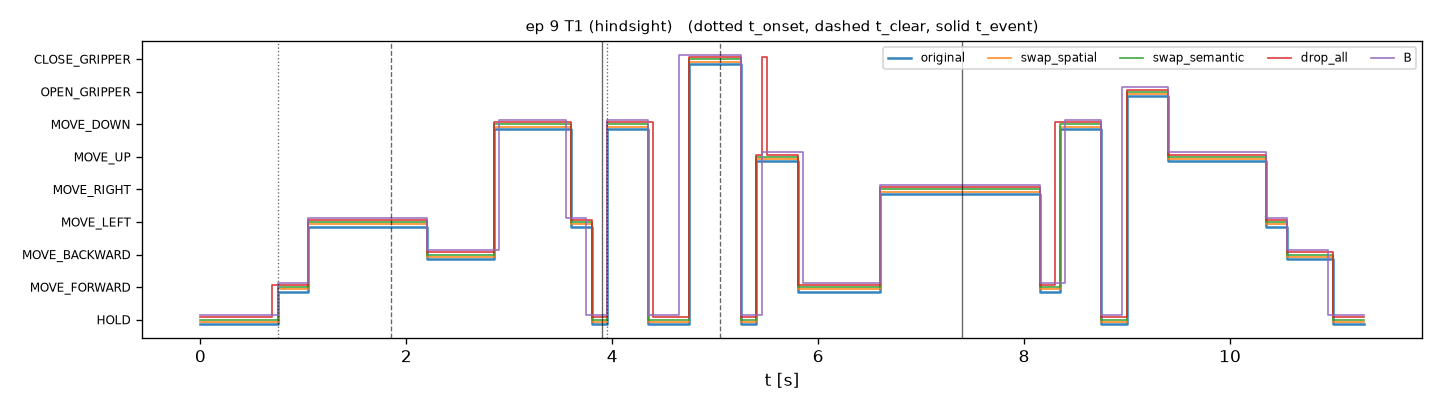
\includegraphics[width=\textwidth]{actions_ep9_T1}
  \caption{Hành động theo thời gian của D trên một episode T1 (episode 9) ở các chế độ: gốc, hoán đổi không gian, hoán đổi ngữ nghĩa, bỏ toàn bộ ý định, và mô hình B. Các vạch dọc là $t_\text{onset}$ (chấm), $t_\text{clear}$ (gạch) và $t_\text{event}$ (liền) của hai cử chỉ chỉ tay.}
  \label{fig:actions-ep9}
\end{figure}

\paragraph{Kiểm chứng quy tắc CGR.} Để tính CGR mà không phải mô phỏng lại mọi khung, khóa luận dùng một quy tắc xấp xỉ: hành động đúng là hành động đưa điểm công cụ về phía mục tiêu mới. Quy tắc này được đối chiếu với expert mô phỏng lại trên 25 khung và khớp ở 19 khung (76\%). Cả 6 khung không khớp đều rơi vào giai đoạn expert mở kẹp trong T3, nơi quy tắc ``đi về phía mục tiêu'' không mô tả đúng hành động mở kẹp. Vì CGR chỉ có ý nghĩa khi ICR đủ lớn, hạn chế này chưa ảnh hưởng tới kết luận ở trên.

\section{Đánh giá vòng kín}
\label{sec:closed-loop-results}

Bảng~\ref{tab:closed-loop} cho tỉ lệ hoàn thành nhiệm vụ trên 120 episode đánh giá.

\paragraph{Expert.} Expert phản hồi sớm đạt CSR 0,892, với các lỗi như sau:
\begin{itemize}
  \item hết thời gian ở T2 và T4;
  \item làm đổ cốc ở T3;
  \item dừng không cần thiết ở T4-neg.
\end{itemize}
Đây là mức tham chiếu của dữ liệu trình diễn.

\paragraph{Hai chính sách học được.} Cả hai đều \textbf{thất bại gần như hoàn toàn}:
\begin{itemize}
  \item B hoàn thành 1/120 episode (CSR 0,008);
  \item D hoàn thành 11/120 episode (CSR 0,092);
  \item gần như mọi thất bại đều do \emph{hết thời gian}.
\end{itemize}
Tỉ lệ thời gian robot đứng yên (IR) cho thấy nguyên nhân: ở vai Instructor, IR là 0,999 với B và 0,918 với D, so với 0,000 của expert. Nghĩa là chính sách gần như đứng yên suốt episode thay vì làm sai.

\paragraph{An toàn.} Về an toàn, cả ba đều không có va chạm (CFR $= 1$). HCS của B (0,979) và D (1,000) cao hơn expert (0,926). Tuy nhiên kết quả này chủ yếu phản ánh việc robot ít chuyển động, không phải chính sách an toàn hơn.

\begin{table}[htbp]
  \centering
  \caption{Tỉ lệ hoàn thành nhiệm vụ (CSR) trong đánh giá vòng kín, 20 episode mỗi nhiệm vụ.}
  \label{tab:closed-loop}
  \begin{tabular}{@{}lccccccc@{}}
    \toprule
    \textbf{Tác tử} & \textbf{T1} & \textbf{T2} & \textbf{T3} & \textbf{T4} & \textbf{T4-neg} & \textbf{T5} & \textbf{Tất cả} \\
    \midrule
    Expert (phản hồi sớm) & 1,00 & 0,85 & 0,85 & 0,85 & 0,85 & 0,95 & 0,892 \\
    B                     & 0,00 & 0,00 & 0,05 & 0,00 & 0,00 & 0,00 & 0,008 \\
    D                     & 0,05 & 0,15 & 0,00 & 0,15 & 0,15 & 0,05 & 0,092 \\
    \bottomrule
  \end{tabular}
\end{table}

\section{Thảo luận}
\label{sec:discussion}

\paragraph{Khoảng cách giữa ngoại tuyến và vòng kín.} Độ chính xác từng bước trên 0,92 nhưng tỉ lệ hoàn thành dưới 0,1 là biểu hiện điển hình của lỗi tích lũy do lệch phân phối~\cite{ross2011dagger}. Trong một episode dài vài trăm bước, chỉ cần chính sách rơi vào một trạng thái mà nó dự đoán \texttt{HOLD}, robot sẽ đứng yên. Trạng thái của robot khi đó không đổi, ảnh camera gần như không đổi, nên quyết định tiếp theo cũng không đổi. Chỉ số IR gần 1 ủng hộ cách giải thích này.

Ngoài ra, dữ liệu trình diễn chứa nhiều giai đoạn mà robot \emph{phải} đứng chờ người, ví dụ khi chờ người ra hiệu xong hay chờ người cầm vật. Những trạng thái chờ này có thể trông rất giống các trạng thái robot cần di chuyển. Vì chính sách không có bộ nhớ và chỉ thực thi một bước mỗi lần, nó khó phân biệt hai loại trạng thái. Hai hướng khắc phục tự nhiên là:
\begin{itemize}
  \item thu thêm dữ liệu có nhiễu theo DART~\cite{laskey2017dart}, hoặc sửa nhãn trên chính trạng thái của chính sách theo DAgger~\cite{ross2011dagger};
  \item kiểm tra lại sự nhất quán giữa đường ống quan sát lúc huấn luyện và lúc chạy vòng kín.
\end{itemize}

\paragraph{Vì sao D bỏ qua thông tin không gian.} Kết quả kiểm tra ngoại tuyến cho thấy D dựa vào nhóm thời gian và chuyển động nhiều hơn nhóm không gian. Một giải thích hợp lý nằm ở chính dữ liệu trình diễn. Expert phản hồi sớm chỉ cam kết với mục tiêu sau khi bằng chứng đã xuất hiện, ở 40\% chuyển động tiết lộ ý định. Tại thời điểm đó, tay người đã hướng rõ về mục tiêu trong ảnh camera \texttt{high}. Như vậy, trong dữ liệu huấn luyện, mục tiêu luôn \emph{nhìn thấy được} từ ảnh vào đúng lúc nó cần cho hành động. Thông tin ý định không gian vì vậy dư thừa so với ảnh, và mạng không có động lực để đọc nó.

Ngược lại, thông tin thời gian (cử chỉ đã đi được bao nhiêu, còn bao lâu nữa) khó đọc từ một ảnh tĩnh, nên được dùng nhiều hơn. Điều này cũng giải thích vì sao lợi ích ngoại tuyến của D tập trung ở T2 và T4, hai nhiệm vụ mà thời điểm quyết định thành bại.

Quan sát này có hệ quả quan trọng cho thiết kế thí nghiệm: \emph{thông tin ý định chỉ có thể giúp khi dữ liệu trình diễn đòi hỏi hành động trước khi ảnh đủ để suy ra mục tiêu}. Các hướng xử lý tiếp theo gồm:
\begin{itemize}
  \item bỏ thời gian chờ 1,6~s trước khi gắp trong chế độ phản hồi sớm, để robot hành động ngay khi có thông tin;
  \item che hoặc làm nhiễu vùng người trong ảnh khi huấn luyện, buộc mạng dùng thông tin ý định;
  \item bật nhánh FiLM để thông tin ý định tác động trực tiếp lên đặc trưng ảnh;
  \item huấn luyện lâu hơn (50\,000 bước).
\end{itemize}

\paragraph{Về câu hỏi Q3.} Với dữ liệu hiện có, câu trả lời cho Q3 là \emph{chưa}: trên dữ liệu phản hồi sớm, D chỉ nhỉnh hơn B 1,2 điểm phần trăm về độ chính xác ngoại tuyến, và không vượt qua kiểm tra ``có dùng thông tin ý định''. D đạt CSR vòng kín cao hơn B (0,092 so với 0,008), nhưng cả hai đều quá xa expert để có thể kết luận về lợi ích của thông tin ý định.

\section{Các kết quả còn chờ}
\label{sec:results-status}

Bảng~\ref{tab:pending} tổng hợp trạng thái của các thí nghiệm.

\begin{table}[htbp]
  \centering
  \caption{Trạng thái các thí nghiệm tại thời điểm viết.}
  \label{tab:pending}
  \small
  \begin{tabularx}{\textwidth}{@{}l l X@{}}
    \toprule
    \textbf{Thí nghiệm} & \textbf{Trạng thái} & \textbf{Ghi chú} \\
    \midrule
    B, D (hindsight)   & đã có & Mục~\ref{sec:training-results}--\ref{sec:closed-loop-results} \\
    A, C               & chưa chạy & dữ liệu phản hồi khi rõ đã thu (274 episode) \\
    D (perfect)        & chưa chạy & nguồn đã cài đặt, đã đo mức khớp (Bảng~\ref{tab:source-agreement}) \\
    D (predicted)      & chưa chạy & cần đo tham số nhiễu từ người thật \\
    Giữ lại theo nhóm  & một phần & mới có loại bỏ từng nhóm (Bảng~\ref{tab:icr}) \\
    \bottomrule
  \end{tabularx}
\end{table}

\todo{Cập nhật chương này khi có kết quả A, C và các nguồn perfect, predicted.}

% !TEX root = ../main.tex
\chapter{KẾT LUẬN}
\label{chap:conclusions}

\section{Kết quả đạt được}

Khóa luận nghiên cứu câu hỏi liệu một chính sách học bắt chước có hưởng lợi từ thông tin tường minh về ý định của con người trong các nhiệm vụ tương tác người -- robot hay không. Các kết quả chính, theo ba đóng góp đã nêu ở Chương~\ref{chap:introduction}, như sau.

\paragraph{Chính sách nhận thức ý định.} Khóa luận đã đạt được:
\begin{itemize}
  \item một hợp đồng dữ liệu cố định cho thông tin ý định, chia theo ba loại ngữ nghĩa, không gian, thời gian và ứng với năm câu hỏi what, who, which, where, when;
  \item ba nguồn sinh thông tin ý định theo hợp đồng (hindsight, perfect, predicted) dùng chung một bộ nhớ mục tiêu;
  \item một bản mở rộng của ACT nhận thông tin ý định dưới dạng token, có dropout theo nhóm thông tin.
\end{itemize}
Cờ giữ vật suy ra từ độ mở kẹp đạt F1 0,979, và tia chỉ tay lệch trung bình $1{,}23^\circ$, cho thấy các thành phần nhân quả của đường ống hoạt động đúng như thiết kế.

\paragraph{Bộ bối cảnh nhiệm vụ.} Năm nhiệm vụ T1--T5 và biến thể T4-neg thuộc ba vai Instructor, Collaborator, Intruder được xây dựng trong MuJoCo, kèm theo:
\begin{itemize}
  \item bố trí bàn được kiểm tra tự động theo tầm với của robot và người;
  \item mô hình người có chuyển động lặp lại được;
  \item danh sách kịch bản cân bằng (280 kịch bản trình diễn, 120 kịch bản đánh giá);
  \item expert ở hai chế độ thời điểm, đạt CSR 0,892 trong đánh giá vòng kín.
\end{itemize}

\paragraph{Quy trình đánh giá.} Quy trình đánh giá gồm hai mức:
\begin{itemize}
  \item \emph{kiểm tra ngoại tuyến} bằng hoán đổi và loại bỏ theo nhóm thông tin (ICR, CGR, tỉ lệ khởi động sớm sai), trả lời trực tiếp câu hỏi chính sách có dùng thông tin ý định hay không;
  \item \emph{đánh giá vòng kín} với các chỉ số tương tác tính từ chuỗi sự kiện.
\end{itemize}

\paragraph{Kết quả thực nghiệm sơ bộ.} Trên cặp mô hình B và D (dữ liệu phản hồi sớm, nguồn hindsight), các kết quả như sau:
\begin{itemize}
  \item thông tin ý định chỉ cải thiện độ chính xác ngoại tuyến 1,2 điểm phần trăm, tập trung ở các nhiệm vụ phụ thuộc thời điểm (T2, T4, T5);
  \item chính sách hầu như bỏ qua thông tin không gian ($\text{ICR} = 0$ khi hoán đổi mục tiêu trước $t_\text{clear}$), và tiêu chí ``có dùng thông tin ý định'' đặt trước không đạt;
  \item trong vòng kín, cả hai chính sách đều xa expert (CSR 0,008 và 0,092), chủ yếu do đứng yên và hết thời gian.
\end{itemize}
Hai phát hiện này tuy là kết quả âm nhưng có giá trị. Chúng cho thấy (i) lợi ích của thông tin ý định chỉ có thể xuất hiện khi dữ liệu trình diễn đòi hỏi hành động \emph{trước} khi ảnh đủ để suy ra mục tiêu, và (ii) cần giải quyết lỗi tích lũy của nhân bản hành vi trước khi so sánh các mô hình bằng tỉ lệ hoàn thành.

\section{Hạn chế}

Khóa luận có các hạn chế sau:
\begin{itemize}
  \item Toàn bộ thí nghiệm thực hiện trong mô phỏng với người được lập trình sẵn, không phản ứng với robot. Kết quả với người thật có thể khác, nhất là khi tương lai của người phụ thuộc vào hành động của robot.
  \item Mới huấn luyện một seed cho mỗi mô hình. Các mô hình A, C và các nguồn perfect, predicted chưa được đánh giá, nên thiết kế $2\times2$ chưa hoàn chỉnh.
  \item Tham số nhiễu của nguồn predicted chưa được đo từ người thật.
  \item Các chỉ số cam kết (AM, WCR, WCD, CRsp) còn bị ảnh hưởng bởi đường đi hình chữ L của robot.
  \item Các chỉ số tương tác được định nghĩa theo tinh thần HRIBench nhưng chưa đối chiếu từng công thức với bài báo gốc.
\end{itemize}

\section{Hướng phát triển}

Các hướng phát triển tiếp theo, theo thứ tự ưu tiên:
\begin{enumerate}
  \item \textbf{Điều chỉnh dữ liệu trình diễn phản hồi sớm} để robot hành động ngay khi có thông tin, thay vì chờ cử chỉ được giữ đủ lâu. Khi đó thông tin ý định thực sự đi trước ảnh camera.
  \item \textbf{Buộc chính sách dùng thông tin ý định}: che hoặc làm nhiễu vùng người trong ảnh khi huấn luyện, bật nhánh FiLM, và huấn luyện lâu hơn.
  \item \textbf{Giảm lỗi tích lũy} bằng dữ liệu có nhiễu theo DART hoặc thu nhãn trên trạng thái của chính sách theo DAgger, sau đó lặp lại đánh giá vòng kín.
  \item \textbf{Hoàn thiện thiết kế $2\times2$} với A và C, nhiều seed, và chuyển dần từ nguồn hindsight sang perfect, predicted để đo khoảng cách giữa thông tin lý tưởng và thông tin dự đoán.
  \item \textbf{Đo nhiễu từ người thật} bằng camera RGB-D và MediaPipe, thay bộ dự báo vận tốc không đổi bằng các mô hình học được như InteRACT, và tiến tới thử nghiệm với người thật.
\end{enumerate}


\printbibliography[heading=bibintoc, title={Tài liệu tham khảo}]

% --- Phụ lục -------------------------------------------------
% \appendix
% \input{appendix/A_ten_phu_luc}

\end{document}
